\documentclass[11pt,letter]{article}
\usepackage[top=0.65in,bottom=0.9in,left=0.85in,right=0.85in]{geometry}

%\def\baselinestretch{1.25}
\def\baselinestretch{1.0}

\usepackage[greek, english]{babel}
\usepackage{multicol}

\usepackage{graphicx}
\usepackage[export]{adjustbox}


% The use of the times package forces the use of the type-1 times
% roman font, but the times roman font does not look nice.
% Besides the times roman font still does not print correctly on
% the dopy printer.
%\usepackage{times}


\usepackage{fancyhdr}
\usepackage{amsmath}
\usepackage{amssymb}
\usepackage{bm}
\usepackage{bbold}
\usepackage{parskip}

\newcommand{\bv}[1]{\ensuremath{\bm{#1}}}
\newcommand{\vo}{\ensuremath{V_{0}}}
\newcommand{\bvo}{\ensuremath{\bv{V}_{0}}}
\newcommand{\er}{\ensuremath{E_{R}}}
\newcommand{\Lc}{\ensuremath{L_{\mathrm{c}}}}
\newcommand{\dsig}[1]{\ensuremath{ \frac{ d\,\sigma_{#1} }{d\,\Omega} }}
\newcommand{\dbl}{\ensuremath{ \uparrow\! \downarrow \, }}
\newcommand{\spup}{\ensuremath{ \uparrow }}
\newcommand{\spdn}{\ensuremath{ \downarrow}}

\begin{document}

\section{One-dimensional optical lattice potential}

The contents of this section follow the derivation found in Sec.~IV~A of
\cite{RevModPhys.78.179}.

The hamiltonian for an atom moving in a 1D lattice potential is 
\begin{equation}
  H_{\text{single,1D}} = 
  - \frac{\hbar^{2}}{2m} \frac{\partial^{2}}{\partial x^{2}} 
  + \vo\sin^{2}(kx) 
 \label{eq:Hsingle1D}
\end{equation}
where $k=2\pi/\lambda$, and $\lambda$ is the wavelength of the lattice laser.
The lattice spacing is $a=\lambda/2$.  If \vo\ is in units of the recoil energy
$\er=\frac{\hbar^{2}k^{2}}{2m}$, then the hamiltonian can be written as
\begin{equation}
\begin{split}
  H_{\text{single,1D}}= &
    -\frac{1}{k^{2}} \frac{\partial^{2}}{\partial x^{2}} 
    + \vo\sin^{2}(kx) \\
  H_{\text{single,1D}} = &
    -\frac{1}{k^{2}} \frac{\partial^{2}}{\partial x^{2}} 
    + \frac{\vo}{4}(2 - e^{2ikx} - e^{-2ikx} )  \\
\end{split}
\end{equation}
The solution to this equation can be found in terms of Bloch states, which are
labeled by their quasimomentum $q$, and their band index $n$ \begin{equation}
  \psi_{q}^{n}(x) = e^{iqx} \sum_{m \in \mathbb{Z}} c_{qm}^{n} e^{imGx}
  \label{eq:blochstate}
\end{equation}
The lattice translation invariant function that typically accompanies $e^{iqx}$
has been written here as a sum of plane waves (labeled by the integer $m$) at
the reciprocal lattice vectors.  This is the Fourier series of any such
periodic function and represents no loss of generality.   The reciprocal
lattice vector  $G=\frac{2\pi}{a}=2k$, where $a=\lambda/2$ is the lattice
spacing.  

Plugging the Bloch states into the hamiltonian and then rearranging some of the
terms in the infinite sum, we get \begin{equation}
\begin{split}
  H_{\text{single,1D}} \psi_{q}(x) = &  
      \sum_{m} \left[(q/k+2m)^{2} 
      + \frac{\vo}{4}(2-e^{2ikx}-e^{-2ikx}) \right]
      c_{qm}^{n} e^{iqx+im2kx} \\ 
  H_{\text{single,1D}} \psi_{q}(x) = &  
      \sum_{m} \left[ \left(  (q/k+2m)^{2} 
      + \frac{\vo}{2} \right) c_{qm}^{n} 
      - \frac{\vo}{4}c_{q,m-1}^{n} - \frac{\vo}{4}c_{q,m+1}^{n} \right] 
      e^{iqx+im2kx} 
\end{split}
\end{equation}
The left hand side of the time-independent Schrodinger equation is simply 
\begin{equation}
  E_{q}^{n}\psi_{q}(x) = \sum_{m} E_{q} c_{qm}^{n} e^{iqx+imGx}
\end{equation}
For the coefficients $c_{qm}^{n}$ to represent an eigenstate of the problem, the
Bloch state needs to satisfy $H\psi_{q}(x) = E_{q}^{n}\psi_{q}(x)$, and since the
plane waves are linearly independent functions this means that 
\begin{equation}
  \left(  (q/k+2m)^{2} + \frac{\vo}{2} \right) c_{qm}^{n}
  - \frac{\vo}{4}c_{q,m-1}^{n} - \frac{\vo}{4}c_{q,m+1}^{n} = E_{q} c_{qm}^{n} 
\end{equation}
The quasimomentum is restricted to the first Brillouin zone, which can be taken
to be between $[-\frac{\pi}{a}, \frac{\pi}{a})$ or  between $[0,\frac{2\pi}{a})$.  
We will express the quasimomentum in units of $\frac{2\pi}{a}=2\pi$, so in the
equation above we will make the replacement $q/k \rightarrow 2q$.  Also in the
equation for the Bloch state $q \rightarrow 2\pi q$ 
 
We then have a linear system of equations which determines the $c_{qm}^{n}$.
The number of equations is infinite, but for our practical purposes we will
truncate it such that $|m|<\mathcal{N}$.  The resulting equations can be
written in matrix form, for example if we select
$\mathcal{N}=2$ 
\begin{equation}
\left[\begin{smallmatrix}\frac{1}{2} V_{{0}} + 4 \left(q -2\right)^{2} & - \frac{1}{4} V_{{0}} & 0 & 0 & 0\\- \frac{1}{4} V_{{0}} & \frac{1}{2} V_{{0}} + 4 \left(q -1\right)^{2} & - \frac{1}{4} V_{{0}} & 0 & 0\\0 & - \frac{1}{4} V_{{0}} & \frac{1}{2} V_{{0}} + 4 q^{2} & - \frac{1}{4} V_{{0}} & 0\\0 & 0 & - \frac{1}{4} V_{{0}} & \frac{1}{2} V_{{0}} + 4 \left(q + 1\right)^{2} & - \frac{1}{4} V_{{0}}\\0 & 0 & 0 & - \frac{1}{4} V_{{0}} & \frac{1}{2} V_{{0}} + 4 \left(q + 2\right)^{2}\end{smallmatrix}\right]
\end{equation}

In the numerical solution that  we implemented we chose $\mathcal{N}=5$,  it
turns out that to accurately obtain the dispersion relationship for the
$n^\mathrm{th}$ band you pretty much only need $\mathcal{N}=n+1$, so using
$\mathcal{N}=5$ is somewhat overkill for us since we will be mostly
concentrated on the lowest band and the first excited band.  

\subsection{Band structure}

We can find the solutions for the set of coefficients $c_{qm}^{n}$ by
diagonalizing the matrix shown above.  The eigenvalues correspond to the
energies $E_{q}^{n}$ as a function of quasimomentum $q$ and band index $n$,
this set of solutions is referred to as the band structure, and we show it for
a 1D lattice as a function of $q$ in Fig.~\ref{fig:bands1d}, and also as a
function of lattice depth in Fig.~\ref{fig:bands1d_V0} 
\begin{figure}
\centering 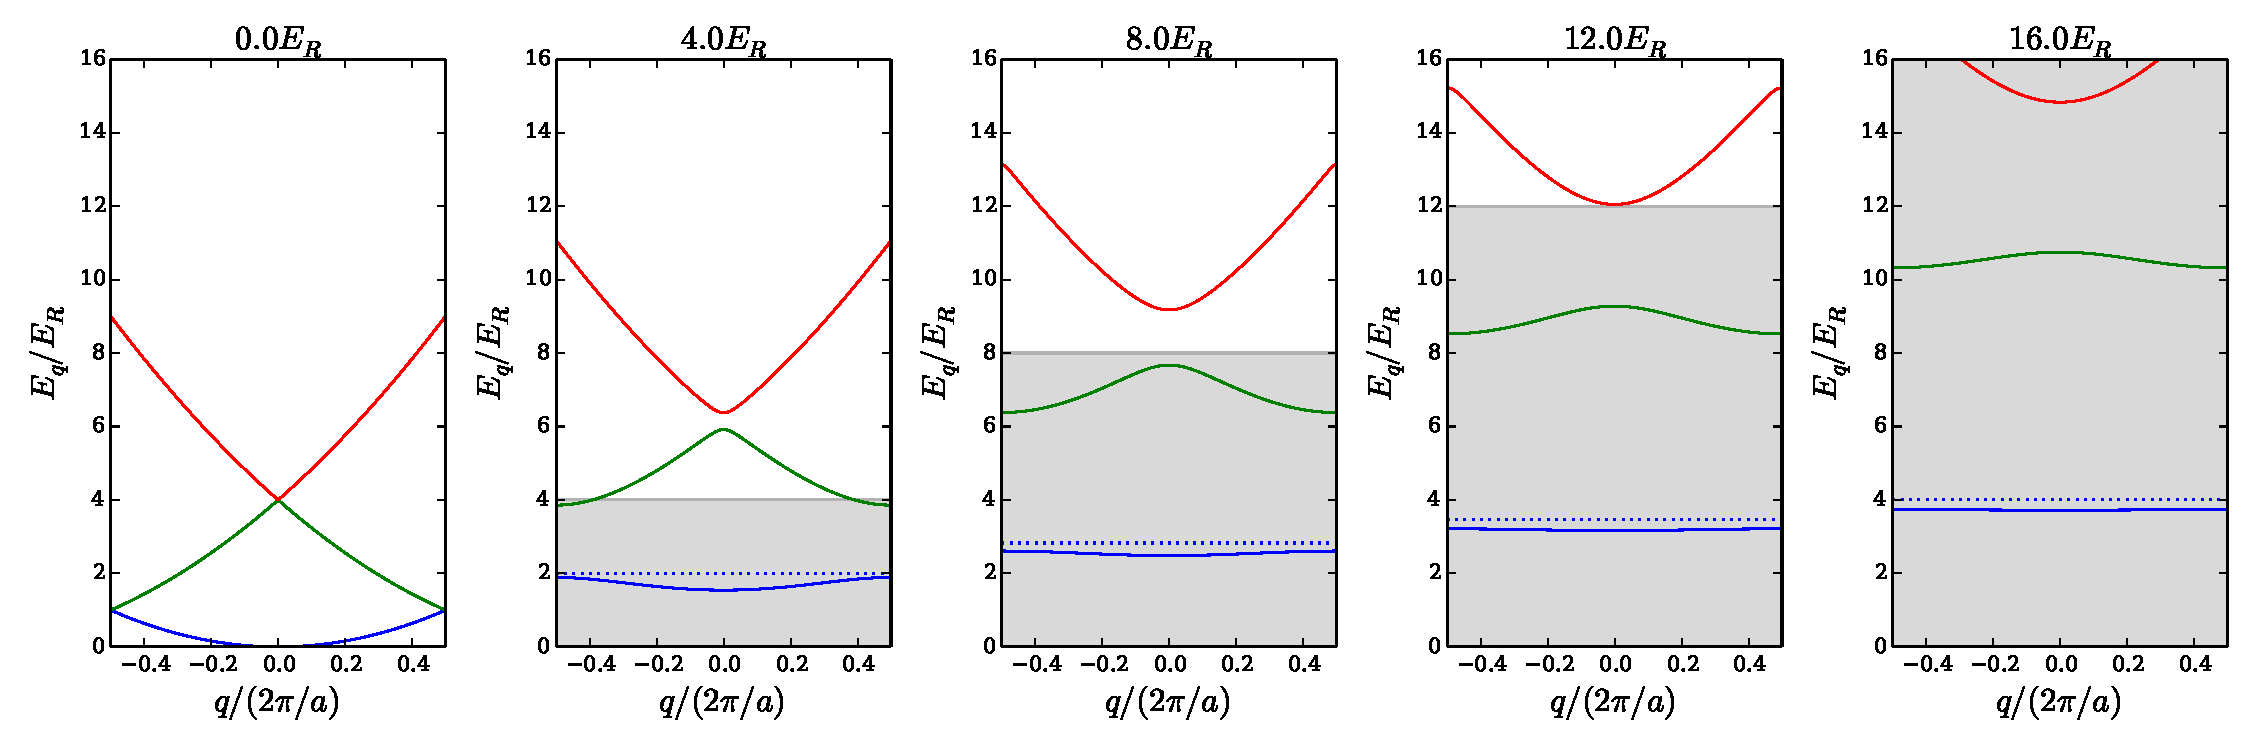
\includegraphics[width=\textwidth]{../BandStructure_figures/bands1d.pdf}
\caption[Band structure in 1D lattice.]{\small Band structure in a 1D optical
lattice.  The depth of the lattice is indicated by the shaded area, and the
energy of the hamonic oscillator ground state in a single lattice site is shown
as a dotted line.  } \label{fig:bands1d}
\end{figure}
\begin{figure}
\centering 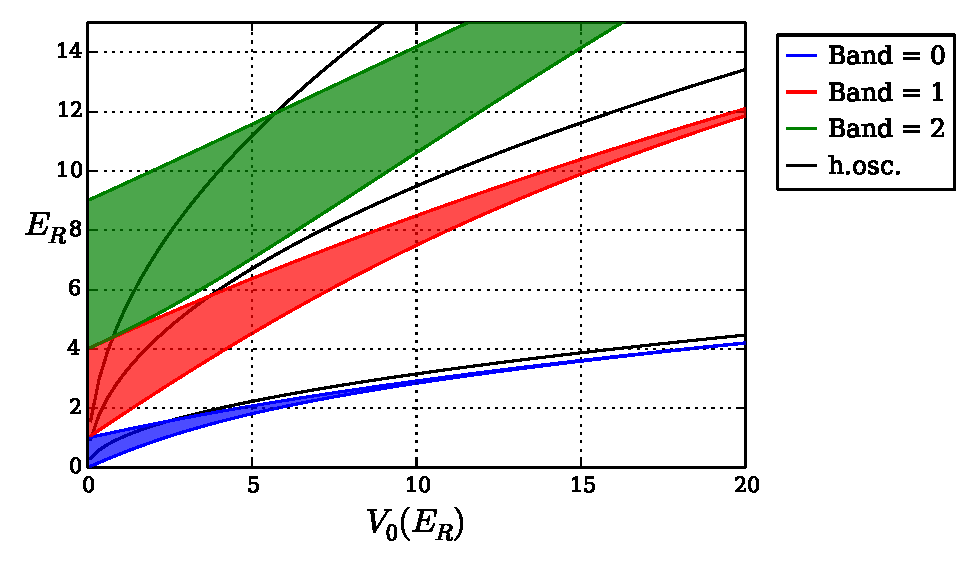
\includegraphics[width=0.6\textwidth]{../BandStructure_figures/bands1d_V0.pdf}
\caption[Band structure in 1D lattice.]{\small Band structure in a 1D optical
lattice.  Each band is indicated by the colored area,  the harmonic oscillator
states in an isolated lattice site are shown as black lines. }
\label{fig:bands1d_V0}
\end{figure}

We mention here that the Schrodinger equation for the hamiltonian in
Eq.~\ref{eq:Hsingle1D}, has solutions called Mathieu functions. 
One can calculate the band structure by using the known properties of the
Mathieu functions, which are avaiable on tables or as functions in some softare
packages (e.g. Mathematica), see for instance the treatement
in~\cite{PhysRev.87.807}. 

\subsection{Eigenstates}
For each energy eigenvalue we have an associated eigenstate  which is defined
in terms of the $c_{qm}^{n}$ by Eq.~\ref{eq:blochstate}.   Typically, numerical
diagonalization routines return the normalized eigenvectors of the matrix in
question,  and for us this means that the coefficients $c_{qm}^{n}$ will
satisfy
\begin{equation}
   \sum_{m} | c_{qm}^{n} |^{2} = 1 
\end{equation} 
This has the implication that the states obtained from Eq.~\ref{eq:blochstate}
will be normalized over a lattice site.  In Fig.~\ref{fig:eigenfuns1d}. we show
the probability density for a lowest band eigenstate as a function of position
in the lattice for various lattice depths.  One can see how, as the lattice
gets deeper, the state becomes more localized around the center of each lattice
site. 
\begin{figure}
\centering 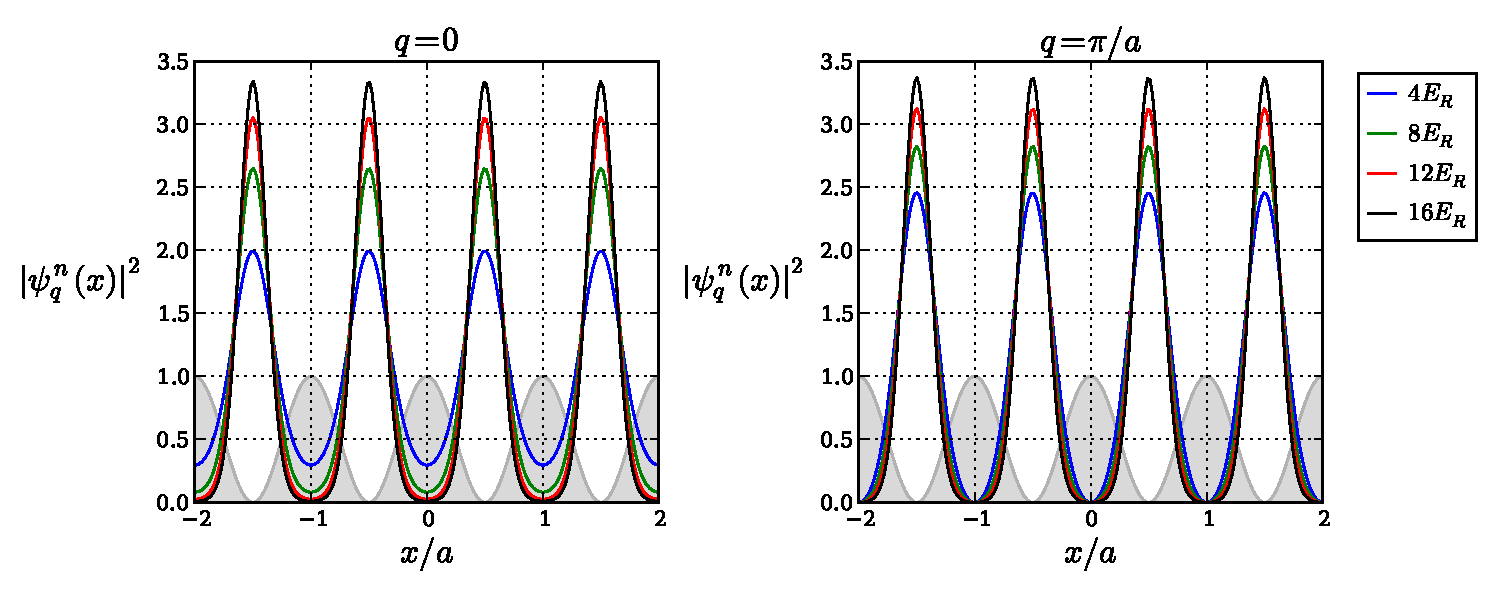
\includegraphics[width=\textwidth]{../BandStructure_figures/eigenfuns1d.pdf}
\caption[Eigenstates in 1D lattice.]{\small Eigenstates of the Hamiltonian in a
1D optical lattice shown for $q=0$ (left) and $q=\pi/a$ (right) for various
lattice depths. The states are normalized so that the integral of the
probability density over one lattice site is equal to one.  The gray shaded
region is shown to indicate the variation of the lattice potential. }
\label{fig:eigenfuns1d}
\end{figure}

\subsection{Wannier states} 
\label{sec:1Dlattice}

It is useful to define a basis of states that are localized around a single
lattice site.  We will see later on that when using such a basis the
hamiltonian for the Hubbard model takes its most familiar form.    The
localized states, centered around the site at $x_{j}$, can be constructed as
the following superposition of eigenstates of the hamiltonian \footnote{In some
treatments (for instance~\cite{salomon2013many}) the Wannier function is
defined with a normalization factor of $\sqrt{N_{s}}$  rather than $N_{s}$ as
shown here.   This is considering eigenfunctions $\psi_{q}^{n}(x)$ which are
normalized when integrating over the full extent in the lattice.  We stick to
the $N_{s}$ normalization factor, without the square root, since the
eigenfunctions that are obtained numerically come out normalized over a lattice
site, as was explained in the previous section.} 
\begin{equation} w^{n}(x-x_{j}) =  \frac{1}{L} \sum_{q}  e^{-i q 2\pi x_{j} }
\psi_{q}^{n}(x) \label{eq:wannier} \end{equation} 
Here we have considered a
finite sized lattice with a total of $L$ sites.  We use the set of unique
quasimomenta defined by $q = \frac{2\pi n}{a} \  \forall n \in \lbrace
0,1,\ldots L-1\rbrace$.  The definition of this set is arbitrary, but there is
no loss of generality.   This becomes clear we insert the
expansion of $\psi_{q}^{n}(x)$ in plane waves into the definition of the
Wannier state. 
\begin{equation}
 w^{n}(x-x_{j}) \equiv w_{j}^{n}(x)= 
    \frac{1}{L} \sum_{q}  
   \sum_{m \in \mathbb{Z}} 
   c_{qm}^{n} 
   e^{-i 2\pi q x_{j} }  
   e^{i 2\pi(q+m)x} 
\end{equation}
The Wannier state is a sum of plane waves, and all plane waves will be covered,
regardless of the set of unique quasimomenta that we decide to consider, since
$m$ runs over all integers.  We will set $x_{j}=0$ for the calculation of the
Wannier function.  WWannier states centered at different lattice sites can be
obtained by translation of the $x_{j}=0$ solution. 
\begin{equation}
  w_{0}^{n}(x)= 
    \frac{1}{L} \sum_{q}  
   \sum_{m \in \mathbb{Z}} 
   c_{qm}^{n} 
   e^{i 2\pi(q+m)x} 
\end{equation}
Since the hamiltonian communtes with the parity operator it is required that
$\psi_{q}^{n}(-x) = \pm \psi_{q}^{n}(x)$ which implies that $c_{qm}^{n} = \pm
c_{q'm'}^{n}$ if  $(q+m) = -(q'+m')$.  Then, the Wannier state becomes
\begin{equation}
  w_{0}^{n}(x)= 
    \frac{1}{L} \left(
   c_{00}^{n} + 
    \sum_{q>0} 
   \sum_{m > 0 } 
   c_{qm}^{n} \left[ e^{i 2\pi(q+m)x} \pm e^{-i 2\pi(q+m)x } \right] \right)
\end{equation}
It is shown in~\cite{Kohn1959} that the maximally localized Wannier states are
obtained if the plus sign is chosen for even bands and the minus sing is chosen
for odd bands.  So, the Wannier states are symmetric for the even bands and
antisymmetric for the odd bands.  \begin{equation}
  w_{0}^{n}(x)= 
    \frac{c_{00}^{n}}{L}
   + 
    \frac{2}{L}
    \sum_{q>0} 
   \sum_{m > 0 } 
   c_{qm}^{n} 
\begin{cases}
\cos[ 2\pi(q+m)x ] & \text{if $n$ even} \\
\sin[ 2\pi(q+m)x ] & \text{if $n$ odd }
\end{cases}
\end{equation}
For $q,m>0$ all the coefficients $c_{qm}^{n}$ will have the same sign, so we
select them to be positive.  

We can now proceed to add up the plane waves to  obtain the Wannier states
which are shown in Fig.~\ref{fig:wannier1d_V0} for various lattice depths.   As
the lattice depth is increased, the Wannier states become more localized.  This
leads to less overlap betweeen Wannier states in adjacent sites, which results
in a reduction of the amplitude for a particle to tunnel from one site to the
next one.   More localized states also imply that the on-site interaction will
be larger, since two particles in the same site will be closer to each other on
average. 
\begin{figure}
\centering 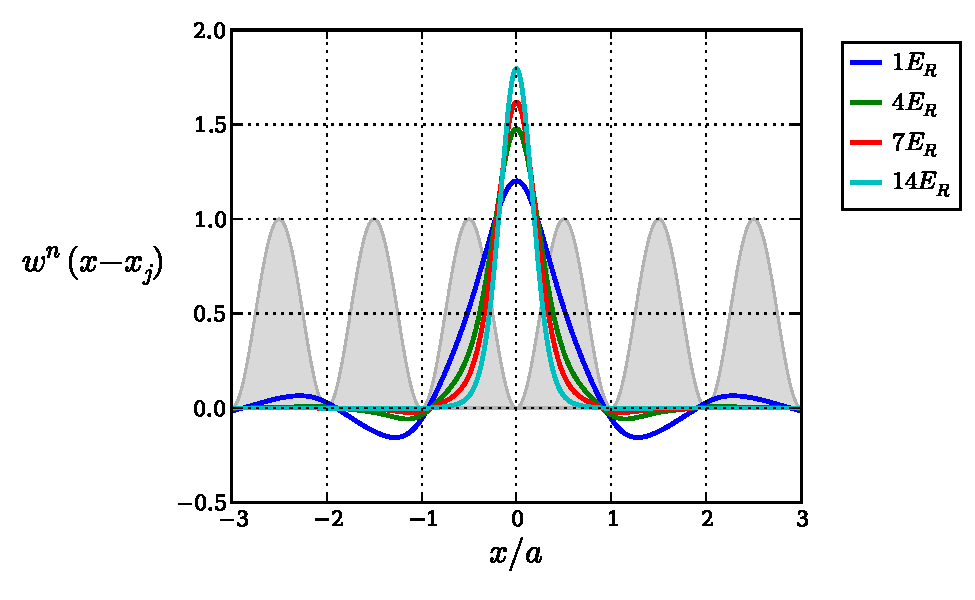
\includegraphics[width=0.6\textwidth]{../BandStructure_figures/wannier1d_V0.pdf}
\caption[Wannier states in 1D lattice for various lattice depths.]{\small
Localized Wannier states in a 1D optical lattice for various lattice depths.
The gray shaded region is shown to  indicate the spatial variation of the
lattice potential.
} \label{fig:wannier1d_V0}
\end{figure}

In Fig.~\ref{fig:wannier1d_bands} we show the Wannier functions for the first
three bands in a 4$E_{R}$ lattice.  
\begin{figure}
\centering 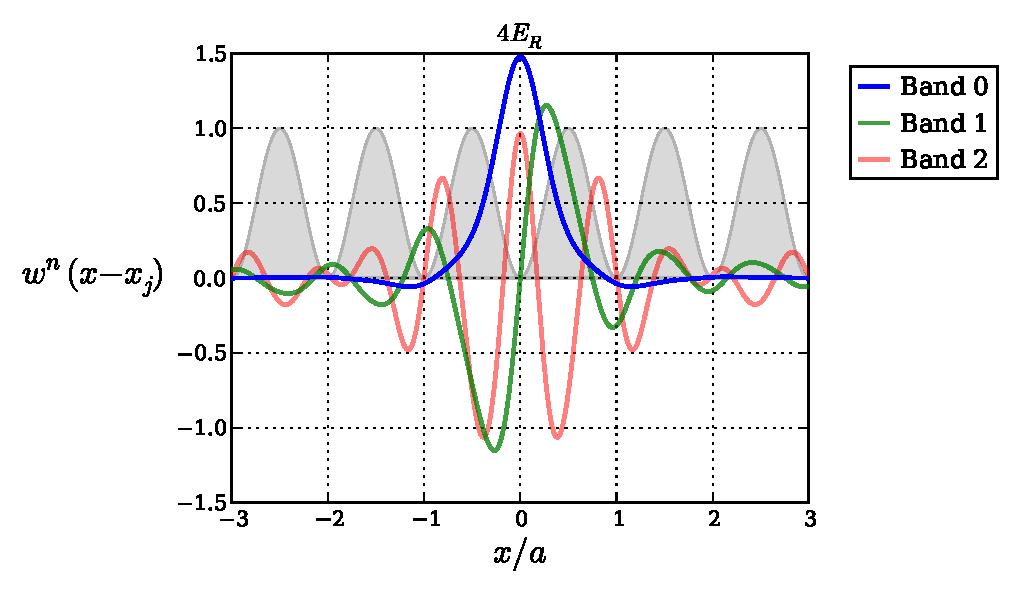
\includegraphics[width=0.6\textwidth]{../BandStructure_figures/wannier1d_bands.pdf}
\caption[Wannier states in 1D lattice for the first three energy bands.]{\small
Localized Wannier states in a 4$E_{R}$ 1D optical lattice for the first three
energy bands.
The gray shaded region is shown to  indicate the spatial variation of the
lattice potential.
} \label{fig:wannier1d_bands}
\end{figure}

\section{Three-dimensional optical lattice potential}

The hamiltonian for an atom moving in a  3D lattice can be separated in the
three spatial coordinates.  So we can use the solutions that were obtained in
the previous section for the 1D lattice and obtain the band structure and the
Wannier states for the 3D lattice.   
The band structure is shown in Fig.~\ref{fig:bands3d_V0}. 
\begin{figure}
\centering 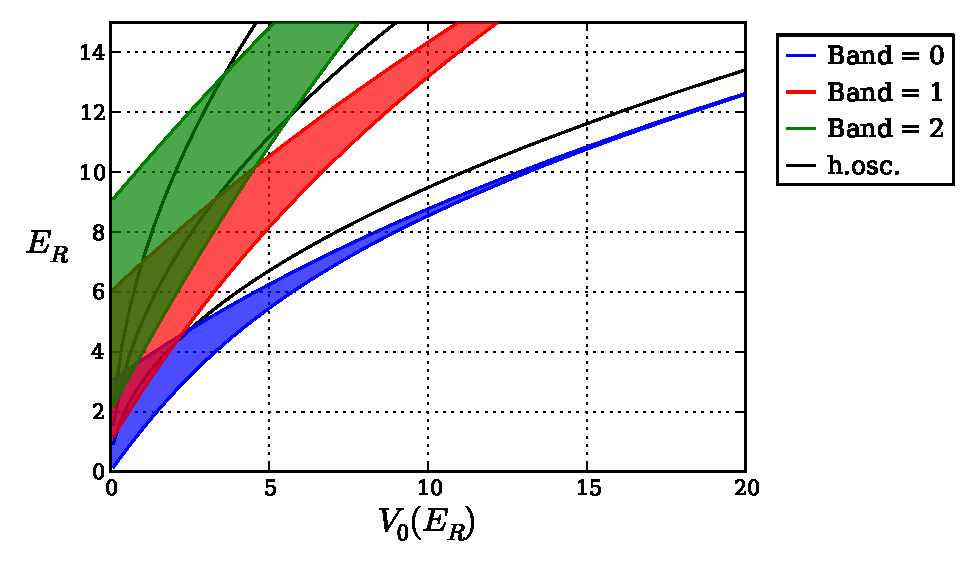
\includegraphics[width=0.6\textwidth]{../BandStructure_figures/bands3d_V0.pdf}
\caption[Band structure in 3D lattice.]{\small Band structure in a 3D optical
lattice.  Each band is indicated by the colored area,  the harmonic oscillator
states in an isolated lattice site are shown as black lines. }
\label{fig:bands3d_V0}
\end{figure}

The Wannier states in a 3D lattice are simply products of the Wannier states in
each of the three spatial coordinates.  They are defined as 
\begin{equation}
 w^{n}(\bv{r}-\bv{r}_{j}) =  \frac{1}{L^{3}} \sum_{\bv{q}} e^{-i \bv{q}\cdot\bv{r}_{j} }
     \prod_{u=x,y,z}  \psi_{q_{u}}^{n_{u}}(u) 
 \label{eq:wannier3D}
\end{equation}
where $L^{3}$ is the total number of sites in the lattice. 

\section{Hubbard hamiltonian}

The many-body Hubbard hamiltonian is 
\begin{equation}
  H =  
-t \sum_{ \langle ij \rangle, \sigma   } 
          a_{i\sigma}^{\dagger}a_{j\sigma} \\
         + U\sum_{i} n_{i\spup} n_{i\spdn}  
\end{equation}
In what follows we will see how to obtain this many-body form starting from the first quantized version of the hamiltonian for a system of $N$ particles. 


The hamiltonian for a single atom in a 3D optical lattice is given by  
\begin{equation}
  H_{\text{single,3D}} = - \frac{\hbar^{2}}{2m} \left( \frac{\partial^{2}}{\partial x^{2}}
                            + \frac{\partial^{2}}{\partial y^{2}}
                            + \frac{\partial^{2}}{\partial z^{2}} \right)
 + \vo\left( \cos^{2}(kx)  + \cos^{2}(ky) + \cos^{2}(kz) \right)
\end{equation}
and when $N$ particles are considered, along with their interactions the
hamiltonian takes a more complicated form \begin{equation}
\begin{split}
  H = & \sum_{l}^{N}\left[ -\frac{\hbar^{2}}{2m} \left( \frac{\partial^{2}}{\partial x_{l}^{2}}
                            + \frac{\partial^{2}}{\partial y_{l}^{2}}
                            + \frac{\partial^{2}}{\partial z_{l}^{2}} \right)
 + \vo\left( \cos^{2}(kx_{l})  + \cos^{2}(ky_{l}) + \cos^{2}(kz_{l}) \right) \right]\\
      &  + \frac{1}{2}\sum_{ l,m, l\neq m}^{N} V_{\mathrm{int}}(\bv{r}_{l},\bv{r}_{m} )\\ 
    = & H_{0} + H_{\text{int}}
 \label{eq:hubbard1st}
\end{split} 
\end{equation} 
where the particles are labeled by indices $l$,$m$, and $V_{\mathrm{int}}$ is
the potential energy of interaction between two partcles.  In the last line we
have defined the more concise notation that splits the Hamiltonian into the
non-interacting ($H_{0}$) and the interacting ($H_{\text{int}}$) parts. Solving
this problem is a daunting task primarily for two reasons:
\begin{enumerate}
    \item The Bose or Fermi statistics of the identical particles under
consideration require the wavefunctions to be symmetrized or antysymmetrized
products of single-particle wavefunctions.     
    \item The interactions between the particles prevent a straightforward
reformulation of the problem as a collection of easier-to-solve single particle
hamiltonians.  
\end{enumerate}

The formalism of many-body theory encapsulates a series of methods to deal with
the two issues mentioned above.   First, the reformulation of the Schrodinger
equation in the language of second quantization provides the advantage that the
statistics are automatically taken into account by the notation, so one can
essentially forget about the the (anti)symmetrization of the many-particle wave
functions.  The small price to pay is that one needs to be very careful and
consistent about the order in which operators show up in the notation, since
the symmetry properties of the resulting states are contained in the
commutation relations defined between the operators.  Furthermore, second
quantization makes it easy to consider the extended Hilbert space where the
number of particles is not fixed, this is known as Fock space. 

For weak interactions, many-body theory provides a solution to the problem in
terms of perturbation expansions for the physical quantities of interest.   The
theoretical formalism also reduces most of the important physical quantities in
terms of certain matrix elements (Green's functions) which allows the user to
concentrate on obtaining such matrix elements which serve as a starting point
for the exploration of the properties of any system.   The complication arises
when the interactions are not weak, and the perturbative approach of the
many-body formalism breaks down.   For this reason, the Hubbard model with strong
interactions (we will quantify the definition of strong later on) has been a
major challenge for theoretical physicists over the last four decades. 
 


\subsection{Second quantization}

The contents of this section follow the treatment in the books by Fetter and
Walecka~\cite{fetter2003quantum} and Schwabl~\cite{schwabl2005advanced}.  

Let's start with a complete orthonormal set of single particle states $\lbrace
|i\rangle \rbrace = \lbrace |1\rangle, |2\rangle, \ldots \rbrace$, using these
states we can write the basis states for the $N$-particle system as
\begin{equation}
   | i_{1}, \ldots i_{\alpha}, \ldots i_{N} \rangle  
\end{equation} 
which represents a state in which particle 1 is in state $i_{1} \in \lbrace
|i\rangle \rbrace$, particle $\alpha$ is in state $i_{\alpha}$ and so on.
These product states are not eigenstates of the permutation operator $P_{ij}$
which interchanges particles $i$ and $j$.  However, starting from the product
states we can obtain the symmetrized (bosons) and antisymmetrized (fermions)
normalized basis states.   

For bosons the normalized symmetrized states are
\begin{equation} 
  | n_{1},  n_{2}, \ldots \rangle = 
  \frac{1}{\sqrt{N!n_{1}!n_{2}!\ldots}} \sum_{P}  P | i_{1},  i_{2}, \ldots i_{N} \rangle
\end{equation} 
where the sum over $P$ runs over all $N!$ elements of the permutation group for
$N$ objects.  In this expression, $n_{1}$ is the number of times that the state
$|1\rangle$ occurs among the $N$ particles,  or in other words, $n_{1}$ is the
number of particles in state $|1\rangle$.  The sum of all occupation numbers
$n_{i}$ must equal the total number of particles, but otherwise there is no
restriction in the occupation number for bosons.

For fermions the normalized antysymmetrized states are written in the form of
Slater determinants: \begin{equation}
\begin{split}
  | n_{1},  n_{2}, \ldots \rangle = &
  \frac{1}{\sqrt{N!}} \sum_{P} (- 1)^{P} P | i_{1},  i_{2}, \ldots i_{N} \rangle \\
  = &
  \frac{1}{\sqrt{N!}}
  \begin{vmatrix}
  |i_{1}\rangle_{1} & |i_{1}\rangle_{2} & \dotsm & |i_{1}\rangle_{N} \\
  \vdots &  \vdots &  \ddots   & \vdots \\
  |i_{N}\rangle_{1} & |i_{N}\rangle_{2} & \dotsm & |i_{N}\rangle_{N} \\
\end{vmatrix}
\end{split} 
  \label{eq:antisymmetrize} 
\end{equation}  
In this case, the product states are multiplied by -1 for odd permutations, and
the occupation numbers $n_{i}$ can only take the values 0 or 1. 

For both bosons and fermions, we can combine the states for $N=0,1,2,\ldots$
particles to obtain a complete orthonormal set of states for arbitrary particle
number.  This set of states, which are referred to as number states, spans what
is called the Fock space.   

We now define the creation  operators for bosons, which allow us to take a
state from the subspace of $N$ particles, to the subspace of $N+1$  particles.
\begin{equation}
 a_{i}^{\dagger} | \ldots, n_{i}, \ldots \rangle  = 
 \sqrt{n_{i}+1}|\ldots, n_{i}+1, \dots\rangle
\end{equation}
It follows that the adjoint of the creation operator is the annihilation
operator and satisfies 
\begin{equation}
a_{i} | \ldots, n_{i}, \ldots \rangle  
=\begin{cases}
\sqrt{n_{i}}|\ldots, n_{i}-1, \dots\rangle
& \text{if $n_{i}\geq 0$},\\
0 & \text{if $n_{i}=0$}
\end{cases}
\end{equation}
The creation and annihilation operators are defined such that one can create
any state starting from the vacuum state $|0\rangle \equiv |0,0,\ldots\rangle$
in which there are no particles at all.  In more formal terms 
\begin{equation}
  | n_{1}, n_{2}, \dots \rangle = \frac{1}{\sqrt{n_{1}!n_{2}!\ldots}} 
   ( a_{1}^{\dagger} ) ^{n_{1}}  
   ( a_{2}^{\dagger} ) ^{n_{2}}  \ldots | 0 \rangle
  \label{eq:numberstate}
\end{equation}
The boson creation and annihilation operators satisfty the Bose communtation
relations 
\begin{equation}
  [a_{i}, a_{j}] = 0 \ \ \ \ \  
  [a_{i}^{\dagger}, a_{j}^{\dagger}] = 0 \ \ \ \ \   
  [a_{i},a_{j}^{\dagger}]=\delta_{ij}
\end{equation}

In the case of fermions we want to also define creation  operators such that
the number states can be written as in Eq.~\ref{eq:numberstate}.    A subtlety
arises in the case of fermions since  the order in which the creation operators
are applied affects the resulting number state\footnote{This is not a problem
in bosons which is seen by looking at Eq.~\ref{eq:numberstate} and recalling
that the Bose commutation relations say that all creation operators commute}.
Take the number state defined in Eq.~\ref{eq:antisymmetrize}.  If we
interchange the state labels 1 and 2 we get 
\begin{equation}
\begin{split}
  | n_{2},  n_{1}, \ldots \rangle = &
  \frac{1}{\sqrt{N!}} \sum_{P} (- 1)^{P} P | i_{2},  i_{1}, \ldots i_{N} \rangle \\
   = & -
  \frac{1}{\sqrt{N!}} \sum_{P} (- 1)^{P} P | i_{1},  i_{2}, \ldots i_{N} \rangle \\ 
   = & -
  | n_{1},  n_{2}, \ldots \rangle 
\end{split}
\label{eq:fermionsign}
\end{equation} 
where the minus sign in the second line is a result of the properties of
determinants, namely you get a minus sign if you exchange two columns. 

If we adopt as a definition of the creation operators the following expression
for the number state \begin{equation}
  | n_{1}, n_{2}, \dots \rangle =  
   ( a_{1}^{\dagger} ) ^{n_{1}}  
   ( a_{2}^{\dagger} ) ^{n_{2}}  \ldots | 0 \rangle \ \ , \ \ \ \ n_{i}=0,1 
  \label{eq:numberstateFermions}
\end{equation}
then using the result of Eq.~\ref{eq:fermionsign} above, the fermion creation
operators must satisfy the following anticommutation relation 
\begin{equation}
 a_{i}^{\dagger}a_{j}^{\dagger} + a_{j}^{\dagger}a_{i}^{\dagger} 
  \equiv [a_{i}^{\dagger}, a_{j}^{\dagger}]_{+} = 0 
\end{equation}
Notice that this also contains the necessary implication that
$(a_{i}^{\dagger})^{2}=0$, which is a manifestation of the Pauli exclusion
principle.  It follows from here that the creation and annihilation operators
for fermions satisfy \begin{equation}
\begin{split}
  a_{i}^{\dagger}| \ldots, n_{i}, \ldots \rangle 
  =  & (1-n_{i})(-1)^{\sum_{k<i} n_{k}} | \ldots, n_{i}+1, \ldots \rangle \\
  a_{i}| \ldots, n_{i}, \ldots \rangle 
  =  & n_{i}(-1)^{\sum_{k<i} n_{k}} | \ldots, n_{i}-1, \ldots \rangle
\end{split} 
\end{equation}
and also that they satisfy the Fermi anticommutation relations 
\begin{equation}
  [a_{i}, a_{j}]_{+} = 0 \ \ \ \ \  
  [a_{i}^{\dagger}, a_{j}^{\dagger}]_{+} = 0 \ \ \ \ \   
  [a_{i},a_{j}^{\dagger}]_{+}=\delta_{ij}
\end{equation}

From now on we shall focus on the case of Fermions, since this is the most
relevant for our experiment.  

\subsection{Operators in second quantization}

So far two great leaps have been taken: 
\begin{enumerate}
 \item We have swept antisymmetrization under the rug by introducing the number
states, defined from the vacuum in terms of creation operators wich satisfy the
Fermi anticommutation reations.  
 \item We started from an $N$ particle hamiltonian, but we have now defined
states that can handle the description of systems with an arbitrary number of
particles 
\end{enumerate}
The two ideas mentioned are related to the states used to describe the system,
now we will turn to the problem of the observables and see how they are handled
in the second quantization.  


Let us consider the following sum over particles $\sum_{\alpha}
|i\rangle_{\alpha} \langle j | _{\alpha} $ and apply it to the number states as
defined in Eq.~\ref{eq:antisymmetrize} 
\begin{equation}
  \left(
   \sum_{\alpha} |i\rangle_{\alpha} \langle j | _{\alpha}  \right)
  | n_{1},  n_{2}, \ldots \rangle = 
  \frac{1}{\sqrt{N!}} \sum_{P} (- 1)^{P} P 
  \left( \sum_{\alpha} |i\rangle_{\alpha} \langle j | _{\alpha} 
   | i_{1},  i_{2}, \ldots i_{N} \rangle \right)
\end{equation}
On the left hand side, for the term in parenthesis not to vanish, there must be
one particle in state $|j\rangle$, so we must have $n_{j}=1$ in the initial
state.  Also, since these are fermions, there can be no particles in state
$|i\rangle$ in the intitial state, so $n_{i}=0$,  or else the Slater
determinant operator will make the state vanish after applying the
$|i\rangle\langle j|$.  If the particle initially in state $|j\rangle$ is
labeled as  $\beta$  then the two mentioned conditions can be embodied as 
\begin{equation}
\begin{split}
  \left(
   \sum_{\alpha} |i\rangle_{\alpha} \langle j | _{\alpha}  \right)
  | n_{1},  n_{2}, \ldots \rangle = &
   n_{j}(1-n_{i}) 
  \frac{1}{\sqrt{N!}} \sum_{P} (- 1)^{P} P \left( 
    |i\rangle_{\beta}\underbrace{ 
   | i_{1},  i_{2}, \ldots i_{N} \rangle}_{\text{wihtout }|j\rangle_{\beta}}  \right) \\
   =&  n_{j}(1-n_{i})
  \frac{1}{\sqrt{N!}}
  \begin{vmatrix}
  |i_{1}\rangle_{1} & |i_{1}\rangle_{2} & \dotsm & |i_{1}\rangle_{N} \\
  \vdots &  \vdots &     & \vdots \\
  |i\rangle_{1} & |i\rangle_{2} & \dotsm & |i\rangle_{N} \\
  \vdots &  \vdots &     & \vdots \\
  |i_{N}\rangle_{1} & |i_{N}\rangle_{2} & \dotsm & |i_{N}\rangle_{N} \\
\end{vmatrix} \\
\end{split} 
\end{equation}
In the determinant of the left the state $|i\rangle$ appears in the
$j^{\text{th}}$ row, so a few rows need to be exchanged to put it in the
correct place according to our sign convention for the number states.
\begin{equation}
\begin{split}
  \left(
   \sum_{\alpha} |i\rangle_{\alpha} \langle j | _{\alpha}  \right)
  | n_{1},  n_{2}, \ldots \rangle = &
  n_{j}(1-n_{i})| \ldots, n_{i}+1, \ldots,  n_{j}-1, \ldots  \rangle \times  
 \begin{cases}
(-1)^{\sum_{k<j} n_{k} + \sum_{k<i}n_{k}  }
& \text{if $i\leq j$},\\
(-1)^{\sum_{k<j} n_{k} + \sum_{k<i}n_{k} -1 } & \text{if $i>j$}
\end{cases}  \\
   = &  a_{i}^{\dagger} a_{j} 
  | n_{1},  n_{2}, \ldots \rangle 
\end{split} 
\end{equation}
where the last equality can be obtained by examining the definition of the
creating and annihilation operators given above. 

After this last step we can establish the important relation
\begin{equation}
   \sum_{\alpha} |i\rangle_{\alpha} \langle j | _{\alpha} = 
     a_{i}^{\dagger} a_{j} 
\end{equation}

We now turn our attention to the operators in the $N$-particle system.
Consider an operator $T$ that is a sum over single particle operators
\begin{equation}
  T = \sum_{\alpha} t_{\alpha}
\end{equation}  
If we insert the completness relation for the single particle states twice in
this sum we have \begin{equation}
\begin{split}
  T = & \sum_{\alpha} \left( \sum_{i} |i\rangle_{\alpha}\langle i |_{\alpha} \right)
        t_{\alpha} \left( \sum_{j} |j\rangle_{\alpha}\langle j |_{\alpha} \right) \\
    = & \sum_{ij}   \langle i | t | j \rangle  \sum_{\alpha} |i\rangle_{\alpha} \langle j |_{\alpha} \\ 
    = & \sum_{ij}   \langle i | t | j \rangle a_{i}^{\dagger} a_{j} \equiv \sum_{ij} t_{ij}   a_{i}^{\dagger} a_{j} 
\end{split}  
\end{equation}

This is the other big leap provided by the second quantization:  the operators
which were written as a sum over particles now are written as a sum of creation
and annihilation operators over single particle states.   

Operators like the potential energy, which are a sum over two-particle (or
many-particle) operators,  can be equally expressed as sums of creation and
annihilation operators.  For a two-body operator we have the expression
\begin{equation}
\begin{split}
F = & \frac{1}{2} \sum_{\alpha\neq\beta} f(\bv{r}_{\alpha}, \bv{r}_{\beta} )  \\
  = & \frac{1}{2} \sum_{ijkm} \langle ij | f | km \rangle a_{i}^{\dagger} a_{j}^{\dagger} a_{m} a_{k} 
\end{split}
\end{equation}

\subsection{Second quantized Hubbard hamiltonian}

The Hubbard hamiltonian in Eq.~\ref{eq:hubbard1st} is a sum of two
single-particle operators and one two-particle operator.  These are
respectively: the kinetic energy, the energy of the atoms in the lattice
potential, and the interactions between the atoms.  As a single-particle basis
we pick the Wannier states that were derived in Section.~\ref{sec:1Dlattice}

In the Hubbard hamiltonian the two single-particle operators are grouped
together to define the non-interacting part of the hamiltonian 
\begin{equation}
\begin{split}
  H_{0} = & \sum_{l}^{N} -\frac{\hbar^{2}}{2m} \left( \frac{\partial^{2}}{\partial x_{l}^{2}}
                            + \frac{\partial^{2}}{\partial y_{l}^{2}}
                            + \frac{\partial^{2}}{\partial z_{l}^{2}} \right)
 + \vo\left( \cos^{2}(kx_{l})  + \cos^{2}(ky_{l}) + \cos^{2}(kz_{l}) \right) \\
       = & \sum_{l}^{N} H_{\text{single,3D}}^{l}
\end{split}
\end{equation}

\subsubsection{Tunneling matrix element, $t$}

IMPORTANT NOTE: In this section I have already restricted the set of states to
only the Wannier states in the lowest band.  I should mention somewhere in this
section that this approximation is taking place. 


$H_{0}$ is a single particle operator, so it's second quantized form is 
\begin{equation}
\begin{split}
  H_{0} = & \sum_{ij} \langle i| H_{\text{single,3D}} |j \rangle a_{i}^{\dagger} a_{j} \\
        = & -\sum_{ij} t_{ij}  a_{i}^{\dagger} a_{j} \\
\end{split}
\end{equation}  
Note that the sign of $t_{ij}$ was picked rather arbitrarily to follow the
usual conventions.  We now proceed to find the value of the matrix element.
We use the definition of the Wannier states given in Eq.~\ref{eq:wannier3D} to
find 
\begin{equation}
\begin{split}
-t_{ij}  
= & 
  \frac{1}{L^{6}}\int \mathrm{d}\bv{r}\ 
     \sum_{\bv{q}'} e^{i \bv{q'}\cdot\bv{r}_{i} }
     \prod_{u'=x,y,z}  \psi_{q'_{u'}}^{n'_{u'}*}(u') 
  \Big( H_{\text{single,3D}}  \Big)
     \sum_{\bv{q}} e^{-i \bv{q}\cdot\bv{r}_{j} }
     \prod_{u=x,y,z}  \psi_{q_{u}}^{n_{u}}(u)\\ 
= &
  \sum_{\bv{q}\bv{q}'}   
  \frac{E_{\bv{q}}^{n}}{L^{6}}
   e^{ i \bv{q}'\cdot\bv{r}_{i} }  e^{ -i \bv{q}\cdot\bv{r}_{j} }
   \int\mathrm{d}\bv{r}\ 
     \prod_{u'=x,y,z}  \psi_{q'_{u'}}^{n'_{u'}*}(u') 
     \prod_{u=x,y,z}  \psi_{q_{u}}^{n_{u}}(u) \\ 
= &
  \sum_{\bv{q}\bv{q}'}   
  \frac{E_{\bv{q}}^{n}}{L^{6}}
   e^{ i \bv{q}'\cdot\bv{r}_{i} }  e^{ -i \bv{q}\cdot\bv{r}_{j} }
   \delta_{\bv{q}\bv{q}'} \delta_{nn'} L^{3} \\
= &
  \frac{1}{L^{3}}
  \sum_{\bv{q}}   E_{\bv{q}}^{n}
   e^{ i \bv{q}\cdot(\bv{r}_{i} - \bv{r}_{j}) } \\
\end{split} 
\end{equation}
We observe that there is no amplitude to go between states that are in two
different bands, as is indicated by the appereance of $\delta_{nn'}$.   In what
follows we will consider only the lowesrt band, $n=0$,  so we will drop the
band index altogether.  This simplification imposes two important requirements
for our system: 
\begin{enumerate}
\item The temperature and the Fermi energy need to be small compared to the
energy gap between the lowest and first excited band.   
\item The interaction energy scale must also be small comapred to the energy
gap between the lowest and first excited band. 
\end{enumerate}

In the 3D lattice, the energy $E_{\bv{q}} = \sum_{u=x,y,z} E_{q_{u}}^{u} $, and by inserting this into the sum for $t_{ij}$ above we find 
\begin{multline}
-t_{ij} =  \frac{1}{L^{3}} \left[ 
          \left(\sum_{q_{x}} E_{q_{x}}^{\text{\tiny 1D}}   e^{ i q_{x} x_{ij} }   \right)
          \sum_{q_{y}} e^{ i q_{y} y_{ij} }   
          \sum_{q_{z}} e^{ i q_{z} z_{ij} }  
   \right. \\
\left. 
          + 
          \sum_{q_{x}} e^{ i q_{x} x_{ij} }  
          \left(\sum_{q_{y}} E_{q_{y}}^{\text{\tiny 1D}}   e^{ i q_{y} x_{ij} }   \right)
          \sum_{q_{z}} e^{ i q_{z} z_{ij} }  
          + 
          \sum_{q_{x}} e^{ i q_{x} x_{ij} }  
          \sum_{q_{y}} e^{ i q_{y} y_{ij} }   
          \left(\sum_{q_{z}} E_{q_{z}}^{\text{\tiny 1D}}   e^{ i q_{z} z_{ij} }   \right)
\right]
\end{multline}
We make use of the identity $\sum_{q_{x}} e^{ iq_{x}(x_{i}-x_{j}) } = L \delta_{x_{i}x_{j}}$, and similarly for $y,z$ to obtain
\begin{equation}
-t_{ij} =  \frac{1}{L} \left[ 
          \left(\sum_{q_{x}} E_{q_{x}}^{\text{\tiny 1D}}   e^{ i q_{x} x_{ij} }   \right)
          \delta_{y_{i}y_{j}}
          \delta_{z_{i}z_{j}}
          + 
          \left(\sum_{q_{y}} E_{q_{y}}^{\text{\tiny 1D}}   e^{ i q_{y} x_{ij} }   \right)
          \delta_{x_{i}x_{j}}
          \delta_{z_{i}z_{j}}
          + 
          \left(\sum_{q_{z}} E_{q_{z}}^{\text{\tiny 1D}}   e^{ i q_{z} z_{ij} }   \right)
          \delta_{x_{i}x_{j}}
          \delta_{y_{i}y_{j}}
\right]
\end{equation}

We see that if $i=j$ we have 
\begin{equation}
  -t_{ii} =  \frac{3}{L} 
          \sum_{q} E_{q}^{\text{\tiny 1D}}  
\end{equation}
This contribution to $H_{0}$ just adds an overall energy (proportional to the
number of particles in the system), so we just ignore it for convenience.
Ignoring this term sets the zero of energy in the problem exactly at the center
of the lowest band.  This will be important in a later section, when we
consider the phase diagram as a function of the chemical potential.   

If on the other hand $i\neq j$, then we see that we can only consider the
posibility that one of the $x_{ij}, y_{ij}, z_{ij}$ is non-zero, otherwise all
three of the terms in the expression above will vanish due to the Kronnecer
delta terms.  The expression for the tunneling matrix elements simplifies to 
\begin{equation}
  t_{ij} = -\frac{1}{L} \sum_{q} E_{q}^{\text{\tiny 1D}} e^{iq \Delta_{ij}} 
\label{eq:tunneling3D}
\end{equation}

where $\Delta_{ij}$ is the distance between sites at $\bv{r}_{i}$ and
$\bv{r}_{j}$, and $r_{ij}$ must be purely directed along $x$, $y$, or $z$.
Also, as in the definition of the 1D Wannier states, the sum over $q$ runs over
the discrete values $q = \frac{2\pi n}{a} \  \forall n \in \lbrace
0,1,\ldots L-1\rbrace$

We point out here that the tunneling matrix element can be computed directly
from the integral \begin{equation}
  -t_{ij} = \int \mathrm{d}\bv{r} \, w_{i}(\bv{r}) H_{\text{single,3D}} w_{j}(\bv{r}) 
\end{equation}
Numerical forms of the Wannier functions and their derivatives are easily
obtained from the formulas in Sec.~\ref{sec:1Dlattice}.   Calculating the
tunneling matrix element from the Wannier functions is computationally more
expensive than obtaining it as a sum over the energy eigenvalues. 

We observe from Eq.~\ref{eq:tunneling3D} that $t_{ij}$ and $E_{q}^{\text{\tiny
1D}}$ are the Fourier series of one another, or in other words that the
relation just shown can be inverted to obtain 
\begin{equation} 
  E_{q}^{\text{\tiny 1D}} = - \sum_{\Delta_{ij}} t_{ij} e^{-iq \Delta_{ij}} 
\end{equation}
In the tight-binding approximation terms for which $i,j$ are not nearest
neighbors are neglected, and  $\Delta_{ij}$ can only take the values $\lbrace
-a, a \rbrace$.  In this case we use $t_{ij}\equiv t$, and $t$ satisfies
\begin{equation}
  E_{q,\text{tb}}^{\text{\tiny 1D}} = -2 t\cos( qa) 
\end{equation}
This gives an expression that relates the bandwidth, $W_{\text{1D}}$, of the 1D
lattice to the tunneling matrix element $t$ 
\begin{equation} W_{\text{1D}}=4t.\end{equation}  
In 3D this becomes
$W_{\text{3D}}= 12t$.


It is useful to find out the range of lattice depths for which the
tight-binding approximation is valid in the optical lattice potential.  To do
this we just need to look at the tunneling matrix elements for beyond
nearest-neighbor tunneling,  this is shown in Fig.~\ref{fig:tightbinding},
which shows that for lattice depths $\gtrsim 5 E_{R}$  we can safely ignore
tunneling beyond nearest neighbors.  
\begin{figure}
\centering 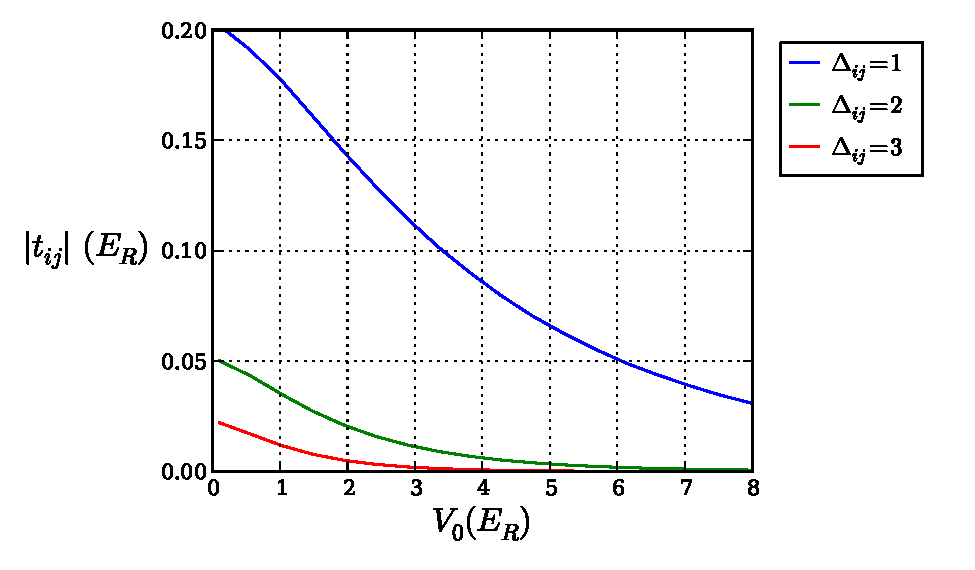
\includegraphics[width=0.6\textwidth]{../BandStructure_figures/tightbinding_V0_interp.pdf}
\caption[Tunneling matrix elements in a 3D lattice.]{\small Tunneling matrix
element in an optical lattice as a function of lattice depth.  Nearest-neighbor
and beyond nearest neighbor matrix elements are shown to illustrate the range
of lattice depths for which the tight-binding limit is a good approximation.
$X_{ij}$ corresponds to the distance between intial and final site in the
tunneling matrix element. 
 } \label{fig:tightbinding}
\end{figure}

Another way of estimating the tunneling matrix element, suggested
in~\cite{Bloch2008}, is by using the relationship $t=W_{\text{1D}}/4$, valid in
the tight-binding limit,  and obtaining the bandwidth from the Mathieu
functions, which are solutions to the Schrodinger equation in a 1D lattice.
This yields the result 
\begin{equation}
 t \simeq \frac{4}{\sqrt{\pi}} \vo^{3/4} \exp(-2\sqrt{\vo}) 
\end{equation} 
where $t$ and $\vo$ are in units of the recoil energy.   The comparision
between the result from Eq.~\ref{eq:tunneling3D} and the  result from the
Mathieu functions is shown in Fig.~\ref{fig:tMathieu}. 
\begin{figure}
\centering 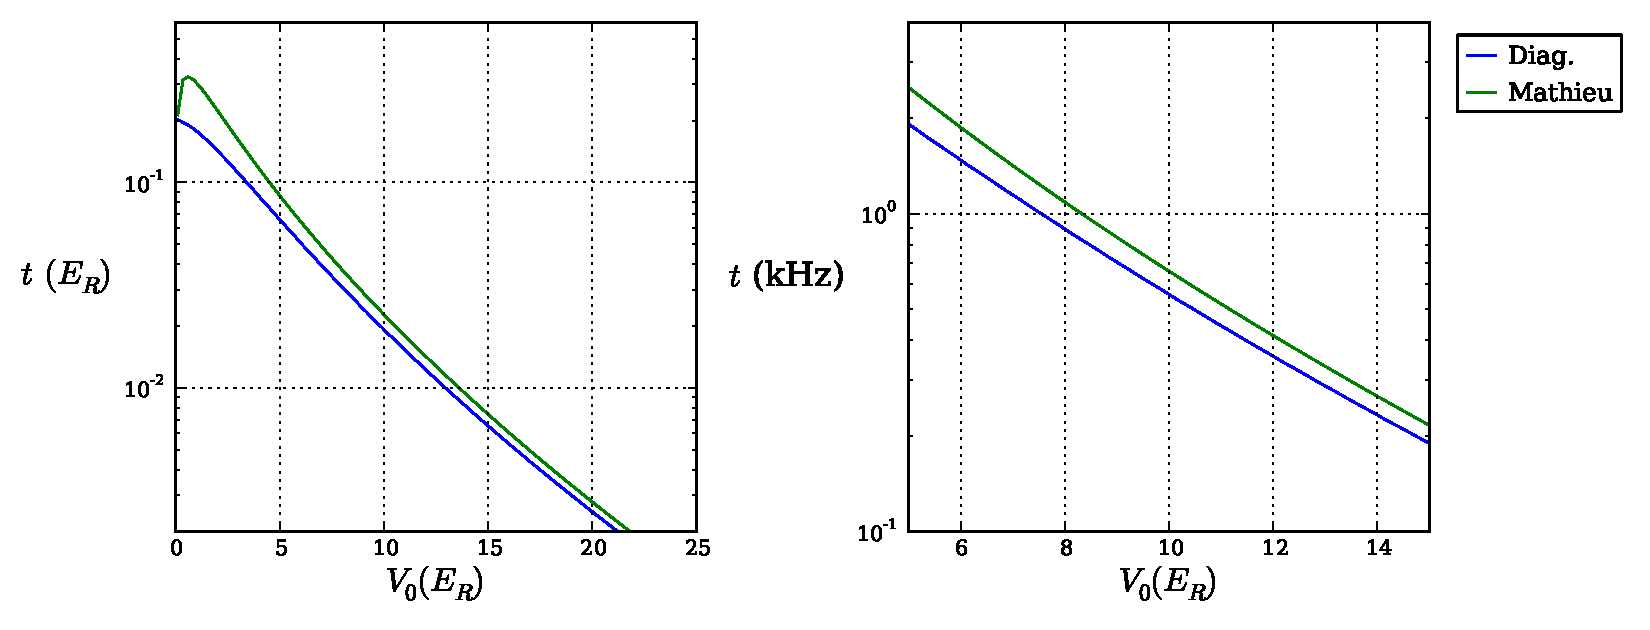
\includegraphics[width=\textwidth]{../BandStructure_figures/tunneling_V0_Mathieu.pdf}
\caption[Nearest neighbor tunneling matrix element]{\small Nearest neighbor
tunneling matrix element in an optical lattice as a function of lattice depth.
Comparison between the result from Eq.~\ref{eq:tunneling3D} and the one
obtained from the Mathieu functions.  The right panel shows the tunneling rate
in kHz for the mass of a $^{6}$Li atom.  } \label{fig:tMathieu}
\end{figure}


Finally, we have the second quantized form of $H_{0}$ in the tight-binding
limit 
\begin{equation}
  H_{0} = -t \sum_{ \langle ij \rangle } a_{i}^{\dagger}a_{j} 
\end{equation}
where the $\langle \rangle$ denote nearest-neighbors, and the creation operator
$a_{i}^{\dagger}$ create particles in the Wannier state localized at site $i$.

Notice that up to now we have ignored the spin part of the wavefunction.   We
can include it easilly by noticing that $H_{0}$ does not act on the spin at
all, so the states $|i\rangle$ and $|j\rangle$ that we have used in the
derivation above need to have the same spin.   With the spin included, our
basis set is now larger which can be taken care of by including a sum over spin
states.   
\begin{equation}
  H_{0} = -t \sum_{ \langle ij \rangle, \sigma=\dbl   } a_{i\sigma}^{\dagger}a_{j\sigma} 
\end{equation}

\subsubsection{On-site interaction energy, $U$}

The interaction part of the hamiltonian for $N$ particles in a 3D lattice is
given by \begin{equation}
    H_{\text{int}} = 
         \frac{1}{2}\sum_{ l,m, l\neq m}^{N} 
         V_{\mathrm{int}}(\bv{r}_{l},\bv{r}_{m} )\\ 
\end{equation}
This is a two-particle operator, and its second quantized form is given by
\begin{equation}
   H_{\text{int}} = \frac{1}{2} \sum_{i,j,k,m} 
           \langle ij | V_{\mathrm{int}} | km \rangle
           a_{i}^{\dagger} a_{j}^{\dagger} a_{m} a_{k}
\end{equation}
where 
\begin{equation}
    \langle ij | V_{\mathrm{int}} | km \rangle =
    \int \mathrm{d}\bv{r}_{1} \int \mathrm{d}\bv{r}_{2} \ \  
    \varphi_{i}^{*}(\bv{r}_{1}) \varphi_{j}^{*}(\bv{r}_{2}) 
    V_{\mathrm{int}}(\bv{r}_{1},\bv{r}_{2}) 
    \varphi_{k}(\bv{r}_{1}) \varphi_{m}(\bv{r}_{2}) 
\end{equation}

The interaction between ultracold atoms can be described in terms of the
$s$-wave scattering length, $a$,  and a pseudopotential given
by~\cite{Bloch2008}
\begin{equation}
    V_{\mathrm{int}}(\bv{r}_{1},\bv{r}_{2}) 
    = \frac{ 4 \pi \hbar^{2} a } { m } \delta(\bv{r}_{1}-\bv{r}_{2}) 
\end{equation}
so the matrix element above can be written as 
\begin{equation}
    \langle ij | V_{\mathrm{int}} | km \rangle =
\frac{ 4 \pi \hbar^{2} a } { m }
    \int \mathrm{d}\bv{r}  \ \  \varphi_{i}^{*}(\bv{r}) \varphi_{j}^{*}(\bv{r}) \varphi_{k}(\bv{r}) \varphi_{m}(\bv{r}) 
\end{equation}
Our basis states, $\varphi$, are the 3D Wannier states defined in
Eq.~\ref{eq:wannier3D}, which are separable in the three spatial coordinates.
We recall that the Wannier states are labeled by the lattice site on which they
are centerend and by their band index.   If we explicitly write out the two
labels in the expression above we obtain
\begin{equation}
    \langle ij | V_{\mathrm{int}} | km \rangle =
\frac{ 4 \pi \hbar^{2} a } { m }
  \prod_{v=x,y,z}
    \int \mathrm{d}v  \ \ 
    w_{i}^{n_{i}}(v) w_{j}^{n_{j}}(v) w_{k}^{n_{k}}(v) w_{m}^{n_{m}}(v)
\end{equation}

The Wannier function along  $x,y,z$ depends on the lattice depth along the
respective coordinate.  We will consider a lattice with different depths along
the three spatial coordinates, $\bvo = ( V_{0x}, V_{0y}, V_{0z} ) $.  At this
point we make the approximation of neglecting all of the off-site interaction
terms, which can be justified by the localized nature of the Wannier states.
Furthermore, we consider only Wannier states in the lowest band, which is valid
for scattering lengths smaller than the single-site harmonic oscillator
length~\cite{Busch1998}.  With this considerations, and also explicitly writing down 
the spin quantum number, which so far was implicit in the indices $ijkm$, we find 
\begin{equation}
\begin{split}
   H_{\text{int}} = &  
           \frac{U}{2}\sum_{\sigma\neq\sigma'}\sum_{i} 
           a_{i\sigma}^{\dagger} a_{i\sigma'}^{\dagger} a_{i\sigma'} a_{i\sigma} \\
     = & 
           \frac{U}{2}\sum_{\sigma\neq\sigma'}\sum_{i}
           n_{i\sigma'} n_{i\sigma}  \\
     = & 
           U\sum_{i}
           n_{i\spup} n_{i\spdn}  
\end{split}
\end{equation}
where now $i$ is an index that runs over lattice sites, and  
\begin{equation}
  U = 
  \frac{ 4 \pi \hbar^{2} a } { m }
   \prod_{v=x,y,z}  \int  w(v) ^{4} \mathrm{d}v  
\end{equation}
In units of $E_{R}$, 
\begin{equation}
  U = \frac{ 8}{ \pi}  \frac{ a_{s} }{a}
   \prod_{v=x,y,z}  \int  w(v) ^{4} \mathrm{d}v  
\end{equation} 
where $a$ is the lattice spacing.  

If the Wannier state is approximated by the Gaussian ground state in the local
oscillator potential of one lattice site, the integral can be carried out
explicity and one gets
~\cite{Bloch2008} 
\begin{equation} 
  U  = \sqrt{ 8\pi } \frac{a_{s}}{a} V_{0}^{3/4} 
\end{equation} 
where, again, the scattering length must be in units of the lattice spacing.

Alternatively we can use the Wannier states which were calculated in
Sec.~\ref{sec:1Dlattice} and obtain a more accurate result.
Figure~\ref{fig:wfactor} shows a comparison of the two methods for a lattice
with $\lambda=1064$\,nm. 
\begin{figure}
\centering 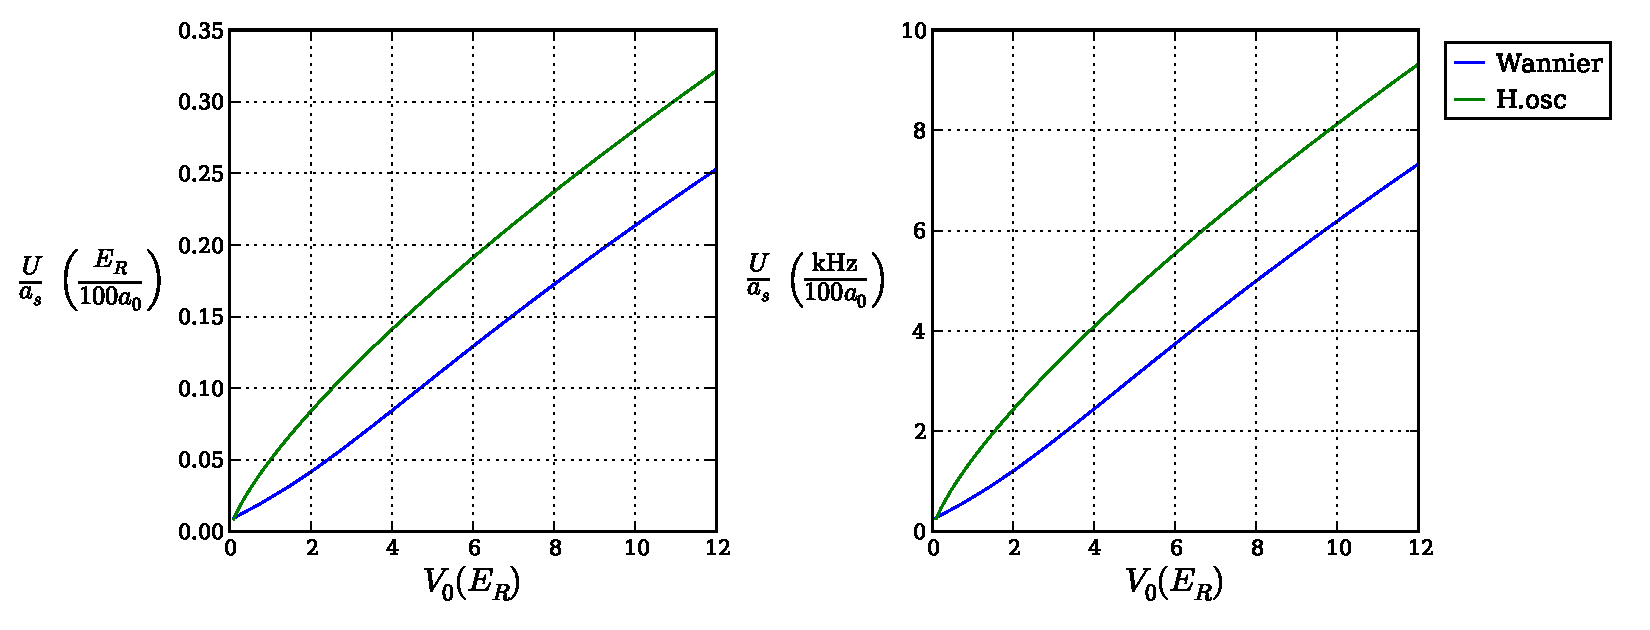
\includegraphics[width=\textwidth]{../BandStructure_figures/wFactor_V0_a0.pdf}
\caption[On-site interactions in a 3D lattice]{\small On-site interactions in a
3D lattice as a function of lattice depth.  Numerical calculation using Wannier
functions compeared to the approximation using harmonic oscillator states.  The
lattice depth is the same in all three directions of the lattice.   The lattice
wavelength is 1064~nm, and it is used to express the interactions in units of
recoils divided by Bohr radius.  The right panel shows it in kHz over Bohr
radius for the mas of a $^{6}$Li atom.} \label{fig:wfactor}
\end{figure}

If the scattering length is too large, and the on-site interaction term
calculated here starts being comparable to the interband spacing then the
single band approximation that we introduced is no longer valid.   One can
treat the problem of two atoms intearcting in the local harmonic oscillator
around a lattice site~\cite{Busch1998}.   Another approach consists of
redefining the single particle basis states (using linear combinations of
Wannier states in different bands) such that the interaction matrix element is
diagonal in the new basis, see for instance~\cite{Jordens2010,Mark2012}. In more formal terms one would find states
\begin{equation}
 \varphi_{i }^{nm}  =  \sum_{st} c_{st}^{nm} w_{i}^{s}(\bv{r} ) w_{i}^{t}(\bv{r})
\end{equation}  
such that 
\begin{equation}
  \langle nm | V_{\mathrm{int}} | op \rangle =  \delta_{n,o}\delta_{m,p}
\end{equation}
The problem of finding the coefficients $c_{st}^{nm}$ can be tackled
numerically by using linear combinations of Wannier states in only
the first few bands. 
    

 

\section{ High-temperature series expansion for the single band Hubbard model }

In the atomic limit, where tunneling between sites is neglected completely, the
Hubbard model can solved exactly.  In this case the tunneling part of the
hamiltonian can be treated as a perturbation and we can gain insight in to the
different phases that the system can exhibit.  This Section follows the
treatment that can be found in~\cite{Henderson1992,Jordens2010}.   

We work in the grand canonical ensemble, so we include a global chemical potential
in the hamiltonian
\begin{equation}
\begin{split}
  H = &  
         \left( U\sum_{i} n_{i\spup} n_{i\spdn}  
         - \mu\sum_{i}( n_{i\spup} + n_{i\spdn} ) \right)
-t \sum_{ \langle ij \rangle, \sigma   } 
          a_{i\sigma}^{\dagger}a_{j\sigma} \\
   = &  H_{0} + H_{1} 
\end{split}
\end{equation}
For the unberturbed part, $H_{0}$, the grand canonical partition function is 
\begin{equation}
 Z_{0} = \text{Tr} e^{-\beta H_{0}} 
\end{equation}
Since the unperturbed part is a sum over sites, the partition function becomes
a product of the single site partition function, $Z_{0} = z_{0}^{k}$, for a
system with $k$ sites.  The single site partition function  is easy to
calculate because the trace runs over the only four possible states in a single
site $\lbrace |0\rangle, |\spup\rangle, |\spdn\rangle, |\dbl\rangle\rbrace$.
\begin{equation}
 z_{0} = 1 + 2 e^{\beta\mu} + e^{\beta (2\mu-U)} = 1 + 2z + z^{2}u 
\end{equation}
where we have defined $z=e^{\beta\mu}$ and $u=e^{-\beta U }$.  Among the
relevant physical quantities that can be obtained are the number of particles,
the number of double occupancies, and the entropy per site.  These are obtained
from the first derivatives of the grand canonical potential, $\Omega$
\begin{equation}
  \Omega = - \frac{\ln Z}{\beta}
\end{equation}
\begin{gather}
  N = -\frac{\partial \Omega}{ \partial \mu }\\
  D = \frac{\partial \Omega}{ \partial U }  \\
  S = -\frac{\partial \Omega}{ \partial T} 
\end{gather}
%\begin{gather}
%  N = -\frac{\partial \Omega}{ \partial \mu }  = z \frac{\partial}{\partial z} \ln Z\\
%  D = \frac{\partial \Omega}{ \partial U }  = u \frac{\partial}{\partial u} \ln Z\\
%  S = -\frac{\partial \Omega}{ \partial T}  = -\beta^{2}  \frac{\partial}{\partial \beta} \ln Z
%\end{gather}
Also, from the second derivatives of the grand potential one can obtain the
fluctuations in any of these quantitites. 

For the full hamiltonian the grand canonical partition function $Z$ can be
expanded in a perturbation series~\cite{Henderson1992} 
\begin{equation}
\begin{split}
  Z = & \text{Tr} e^{-\beta H}  \\
    = & Z_{0} \left[ 1 + 
        \sum_{n=1}^{\infty} (-1)^{n} 
        \int_{0}^{\beta} d\tau_{1} \int_{0}^{\tau_{1}} d\tau_{2} 
        \dotsm \int_{0}^{\tau_{n-1}} d\tau_{n} 
        \langle
              \tilde{H}_{1}(\tau_{1}) 
              \tilde{H}_{2}(\tau_{2})  \dotsm
              \tilde{H}_{n}(\tau_{n})  \rangle 
              \right] 
\end{split}
\end{equation} 
where the thermal expectation value is taken with the
unperturbed part of the hamiltonian
\begin{equation}
\langle A \rangle = \text{Tr} ( e^{\beta H_{0} } A ) / Z_{0} 
\end{equation}
and the tilde means that the operator is evaluated in the interaction picture
for the imaginary time in parenthesis: 
\begin{equation}
 \tilde{H}_{1}(\tau) = e^{\tau H_{0}} H_{1} e^{-\tau H_{0}} 
\end{equation}
Given the series expansion for $Z$, the grand potential is 
\begin{equation}
 -\beta \Omega = Z_{0} + 
        \sum_{n=1}^{\infty} (-1)^{n} 
        \int_{0}^{\beta} d\tau_{1} \int_{0}^{\tau_{1}} d\tau_{2} 
        \dotsm \int_{0}^{\tau_{n-1}} d\tau_{n} 
        \langle
              \tilde{H}_{1}(\tau_{1}) 
              \tilde{H}_{2}(\tau_{2})  \dotsm
              \tilde{H}_{n}(\tau_{n})  \rangle 
\end{equation}

One can see that the $n^{th}$ term in the expansion has $n$ copies of the
tunneling part of the hamiltonian.  Each  application of $H_{1}$ in the thermal
average results in a particle tunneling to a neighboring site, so we see that
there will be a contribution to the expansion only if after $n$ tunneling
events all the particles come back to their original sites.  A direct
consequence of this is that the first order term in the expansion vanishes.
The second order in the expansion corresponds to particles tunneling one site
over and then coming back.  Higher order terms can be represented by diagrams,
to make them easier to keep track off.  The contribution from orders up to
$n=9$ is shown in~\cite{Henderson1992}.  Here we will use up to the second
order term to illustrate the phases that appear in the system.  

The grand potential to second order is~\cite{Henderson1992,Jordens2010} 
\begin{equation}
-\beta \Omega_{2} = k \ln z_{0} + k \left( \frac{\beta t }{z_{0}} \right)^{2} m 
        \left( z + z^{3} u + 2z^{2} \frac{1-u}{\beta U} \right) 
\end{equation} 
where $m$ is the number of nearest neighbors for each lattice site, which in
the simple cubic case is $m=6$.  We see that the grand potential is
proportional to the number of lattice sites, so we will obtain all the
thermodynamic quantities per lattice site. 

The resulting phase diagram is shown in Fig.~\ref{fig:highTphases}.  NOTE FOR
GROUP MEETING:  I intend to write some text that discusses the relevant phases
in this phase diagram.  I will discuss them in the presentation in the group
meeting and add the explanatory text in this document later on.  
\begin{figure}
\centering 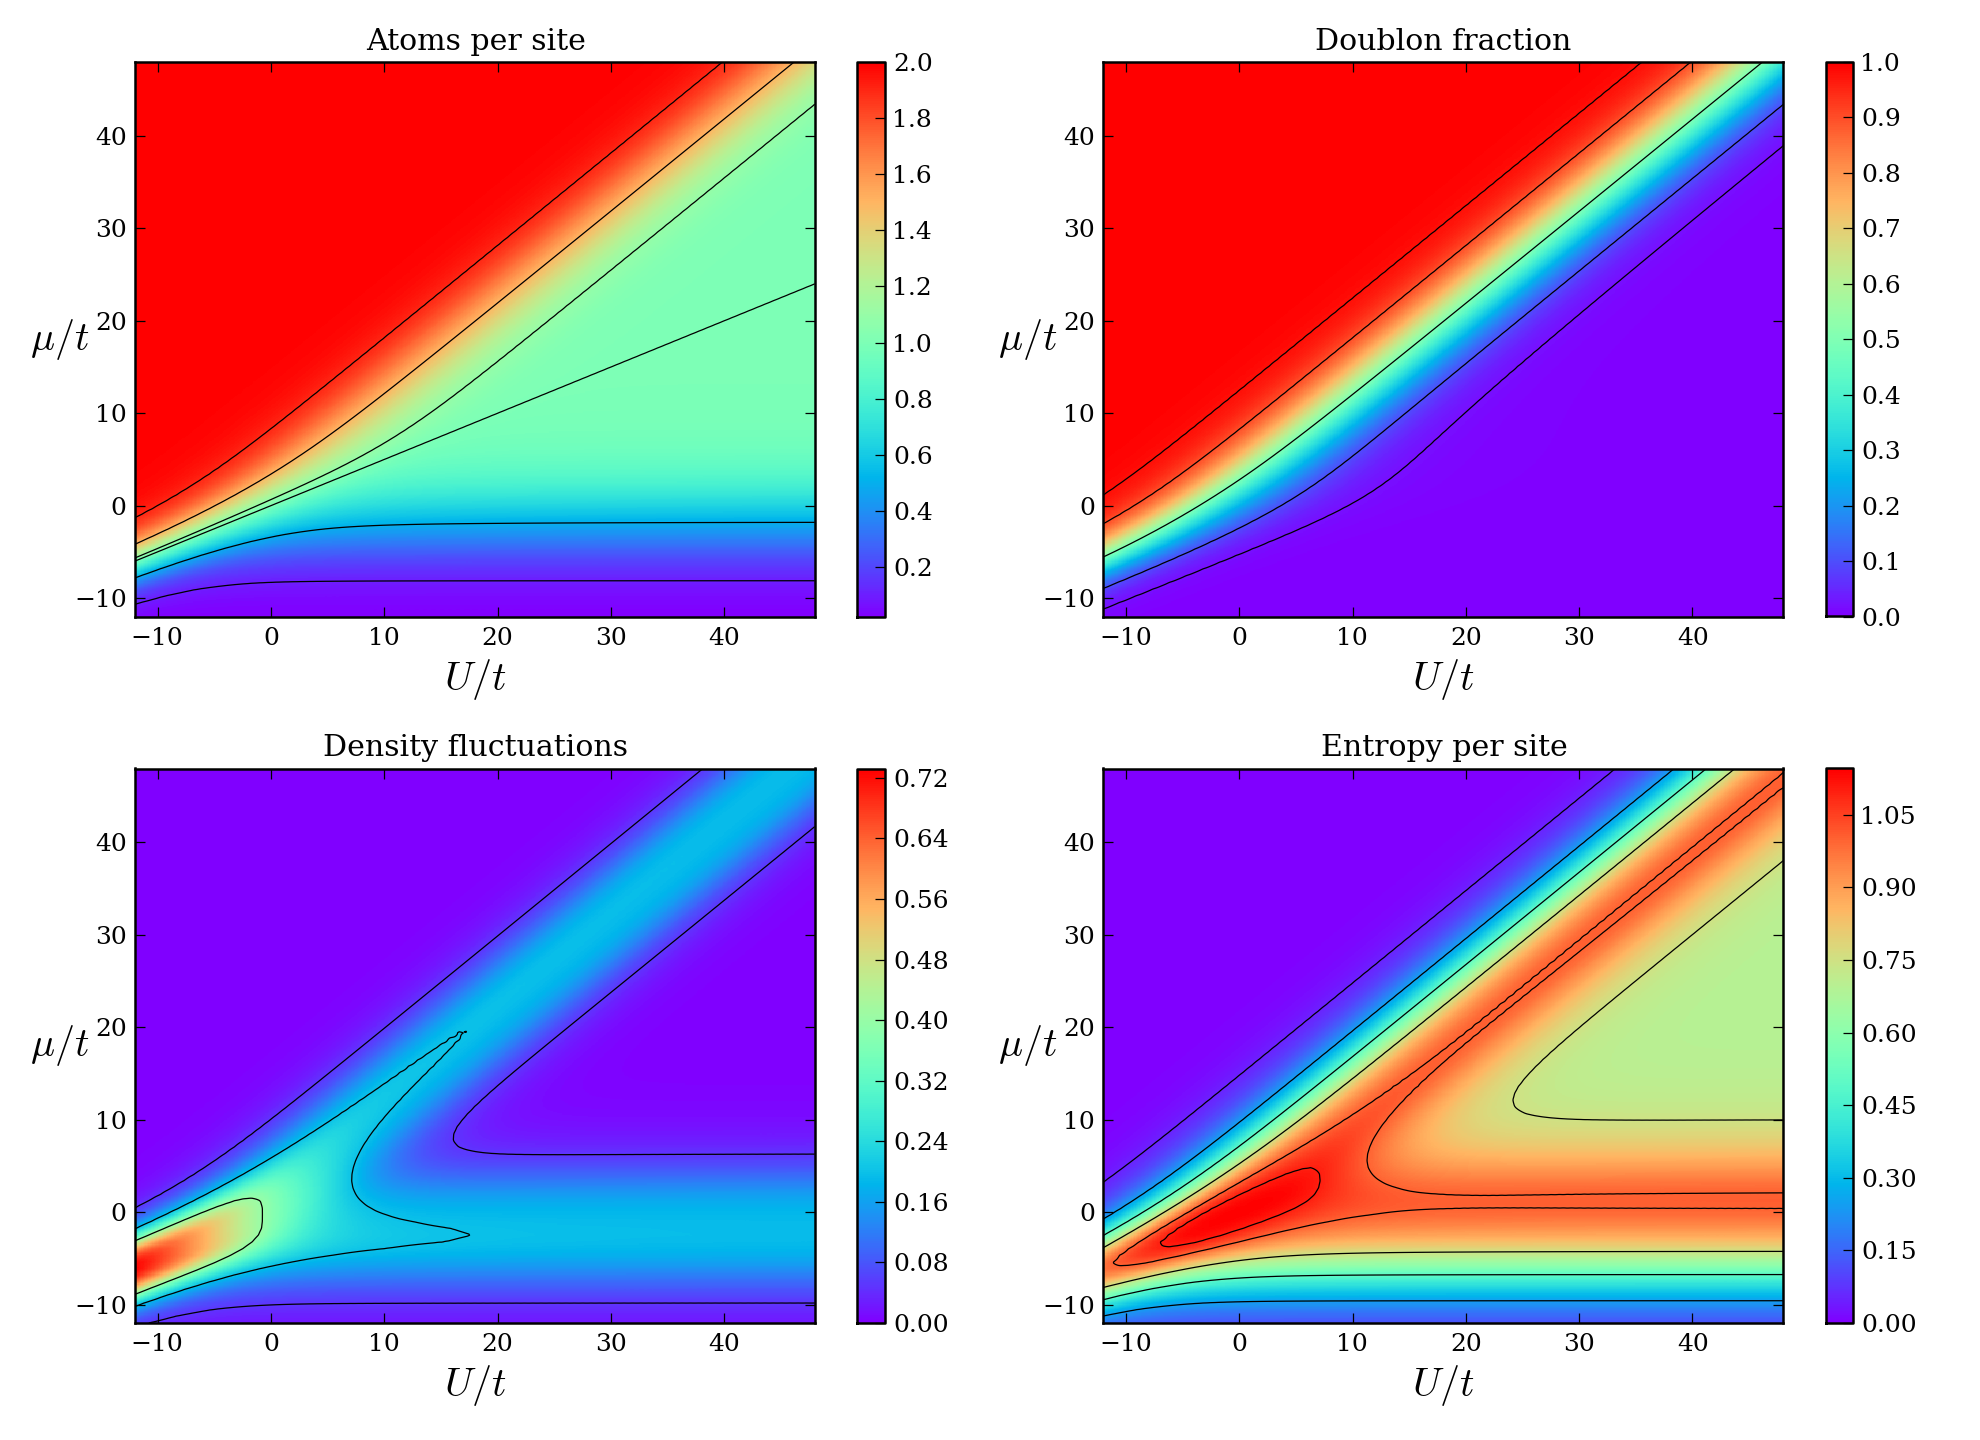
\includegraphics[width=\textwidth]{../HighT_figures/phases2p5.png}
\caption[High temperature phase diagram of the Fermi-Hubbard model]{\small 
High temperature phase diagram of the Fermi-Hubbard model calculated using only the second order in the perturbation series. 
} \label{fig:highTphases}
\end{figure}

\subsection{Thermodynamics at colder temperatures, apparoach to the N\'{e}el transition}

In this section we show the phase diagram for the Fermi-Hubbard model at lower
temperatures, which are beyond the scope of the perturbation expansion shown in
the previous section.   The phase diagram was calculated in~\cite{Fuchs2011} by
using cluster dynamical mean-field theory, and they have made their results
available in the supplementary material accompanying their paper.  In
Figures~\ref{fig:fuchs10, fig:fuchs1, fig:fuchs03} we show the resulting phase
diagram for $T/t=$ 10, 1, and 0.3 respectively.

\begin{figure}
\centering 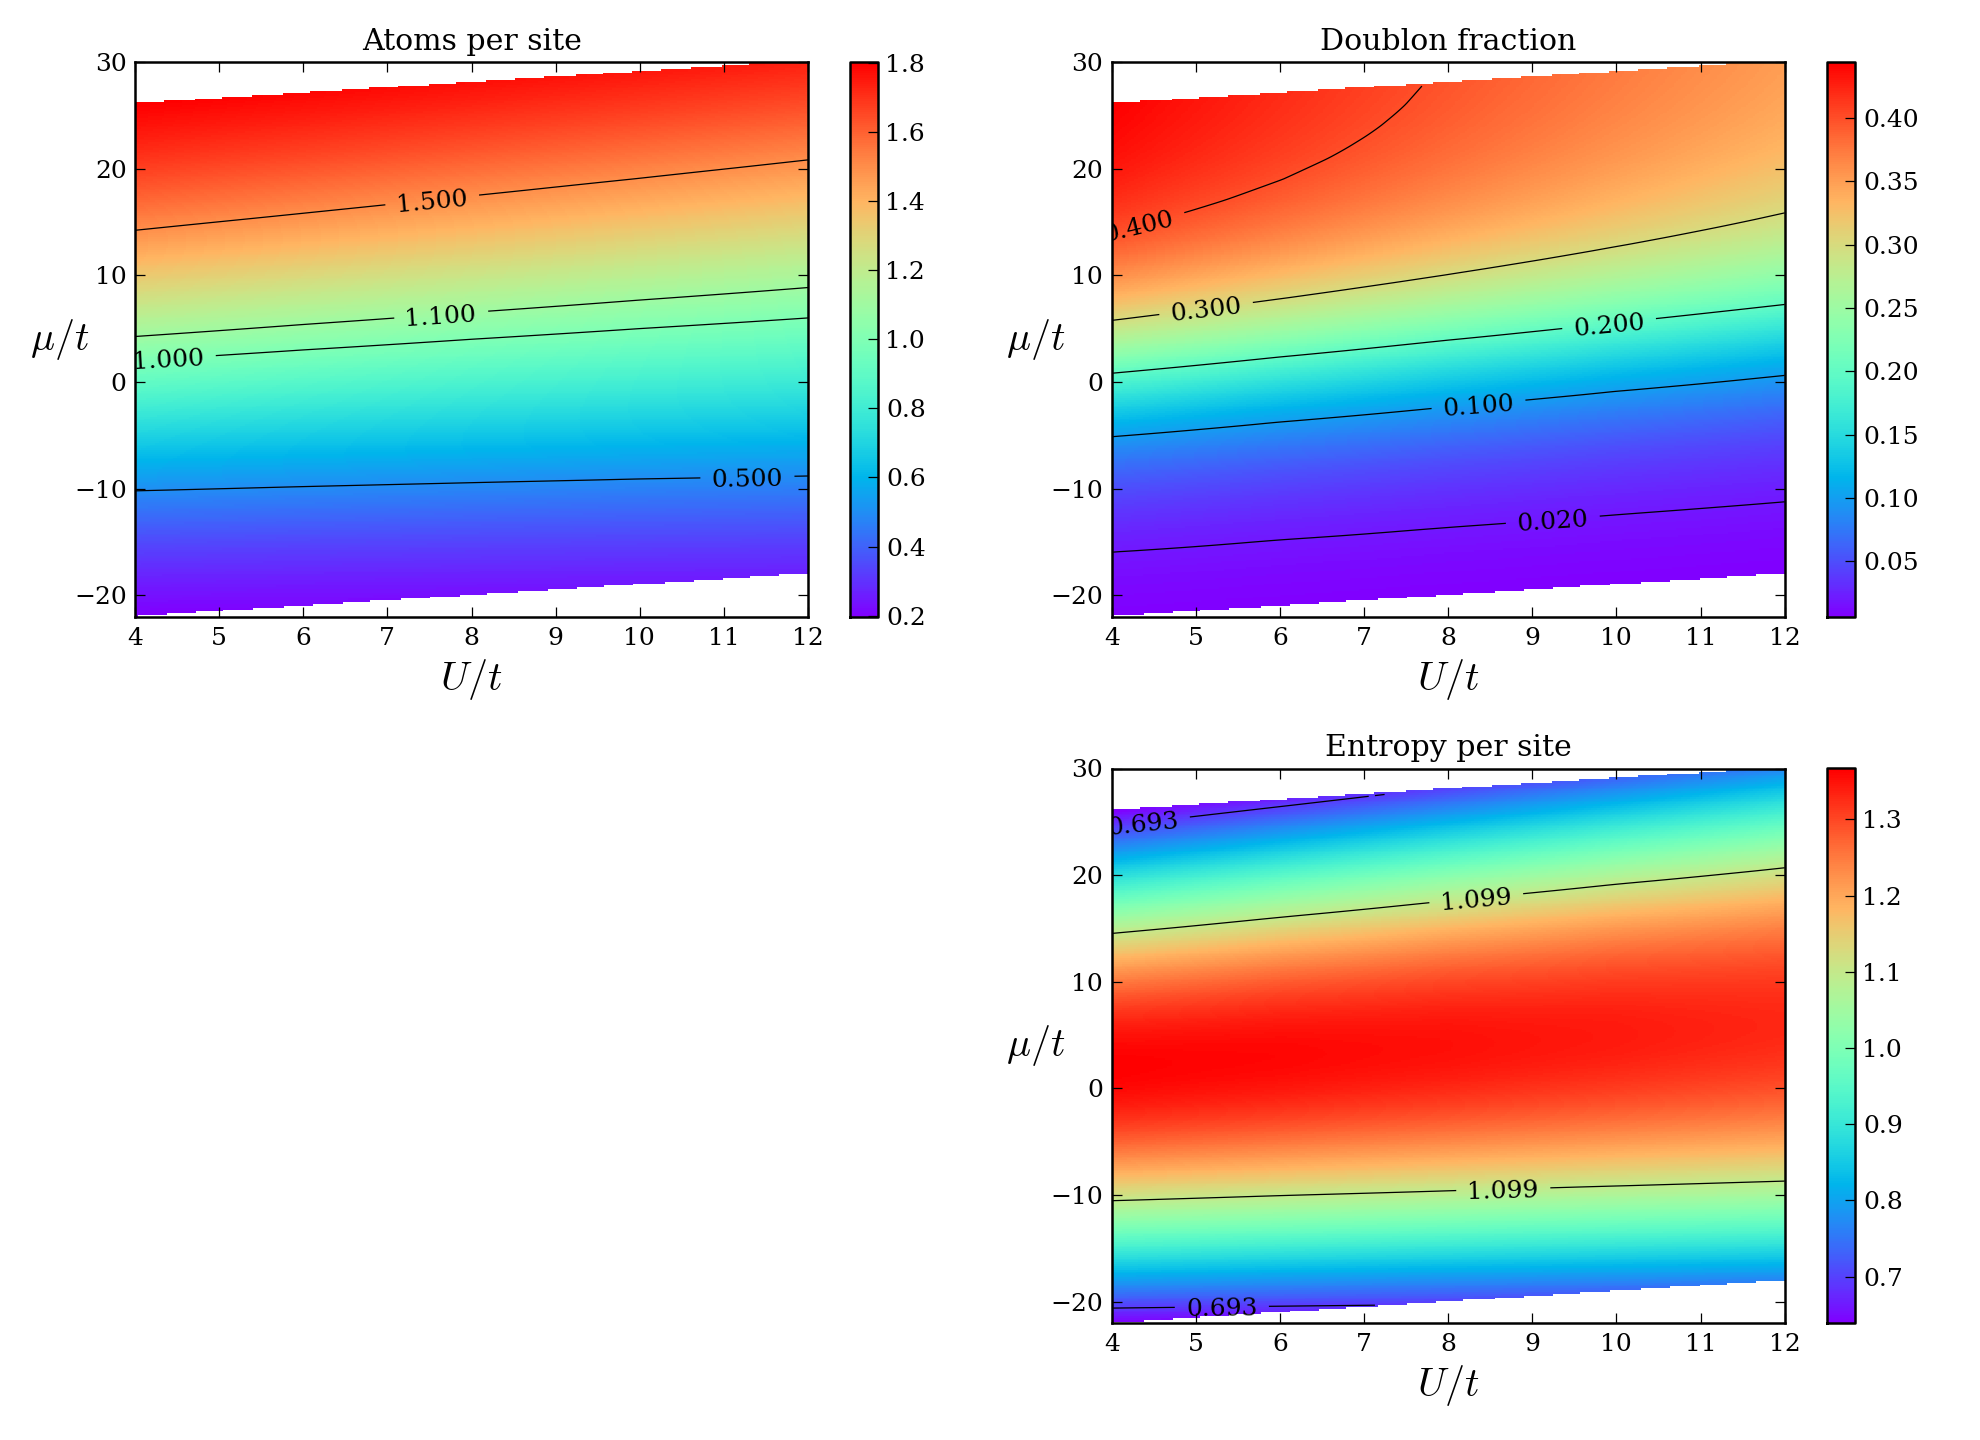
\includegraphics[width=\textwidth]{../HighT_figures/FUCHS_phasesT=100.png}
\caption[Low temperature phase diagram of the Fermi-Hubbard model]{\small
From~\cite{Fuchs2011}} \label{fig:fuchs10}
\end{figure}

\begin{figure}
\centering 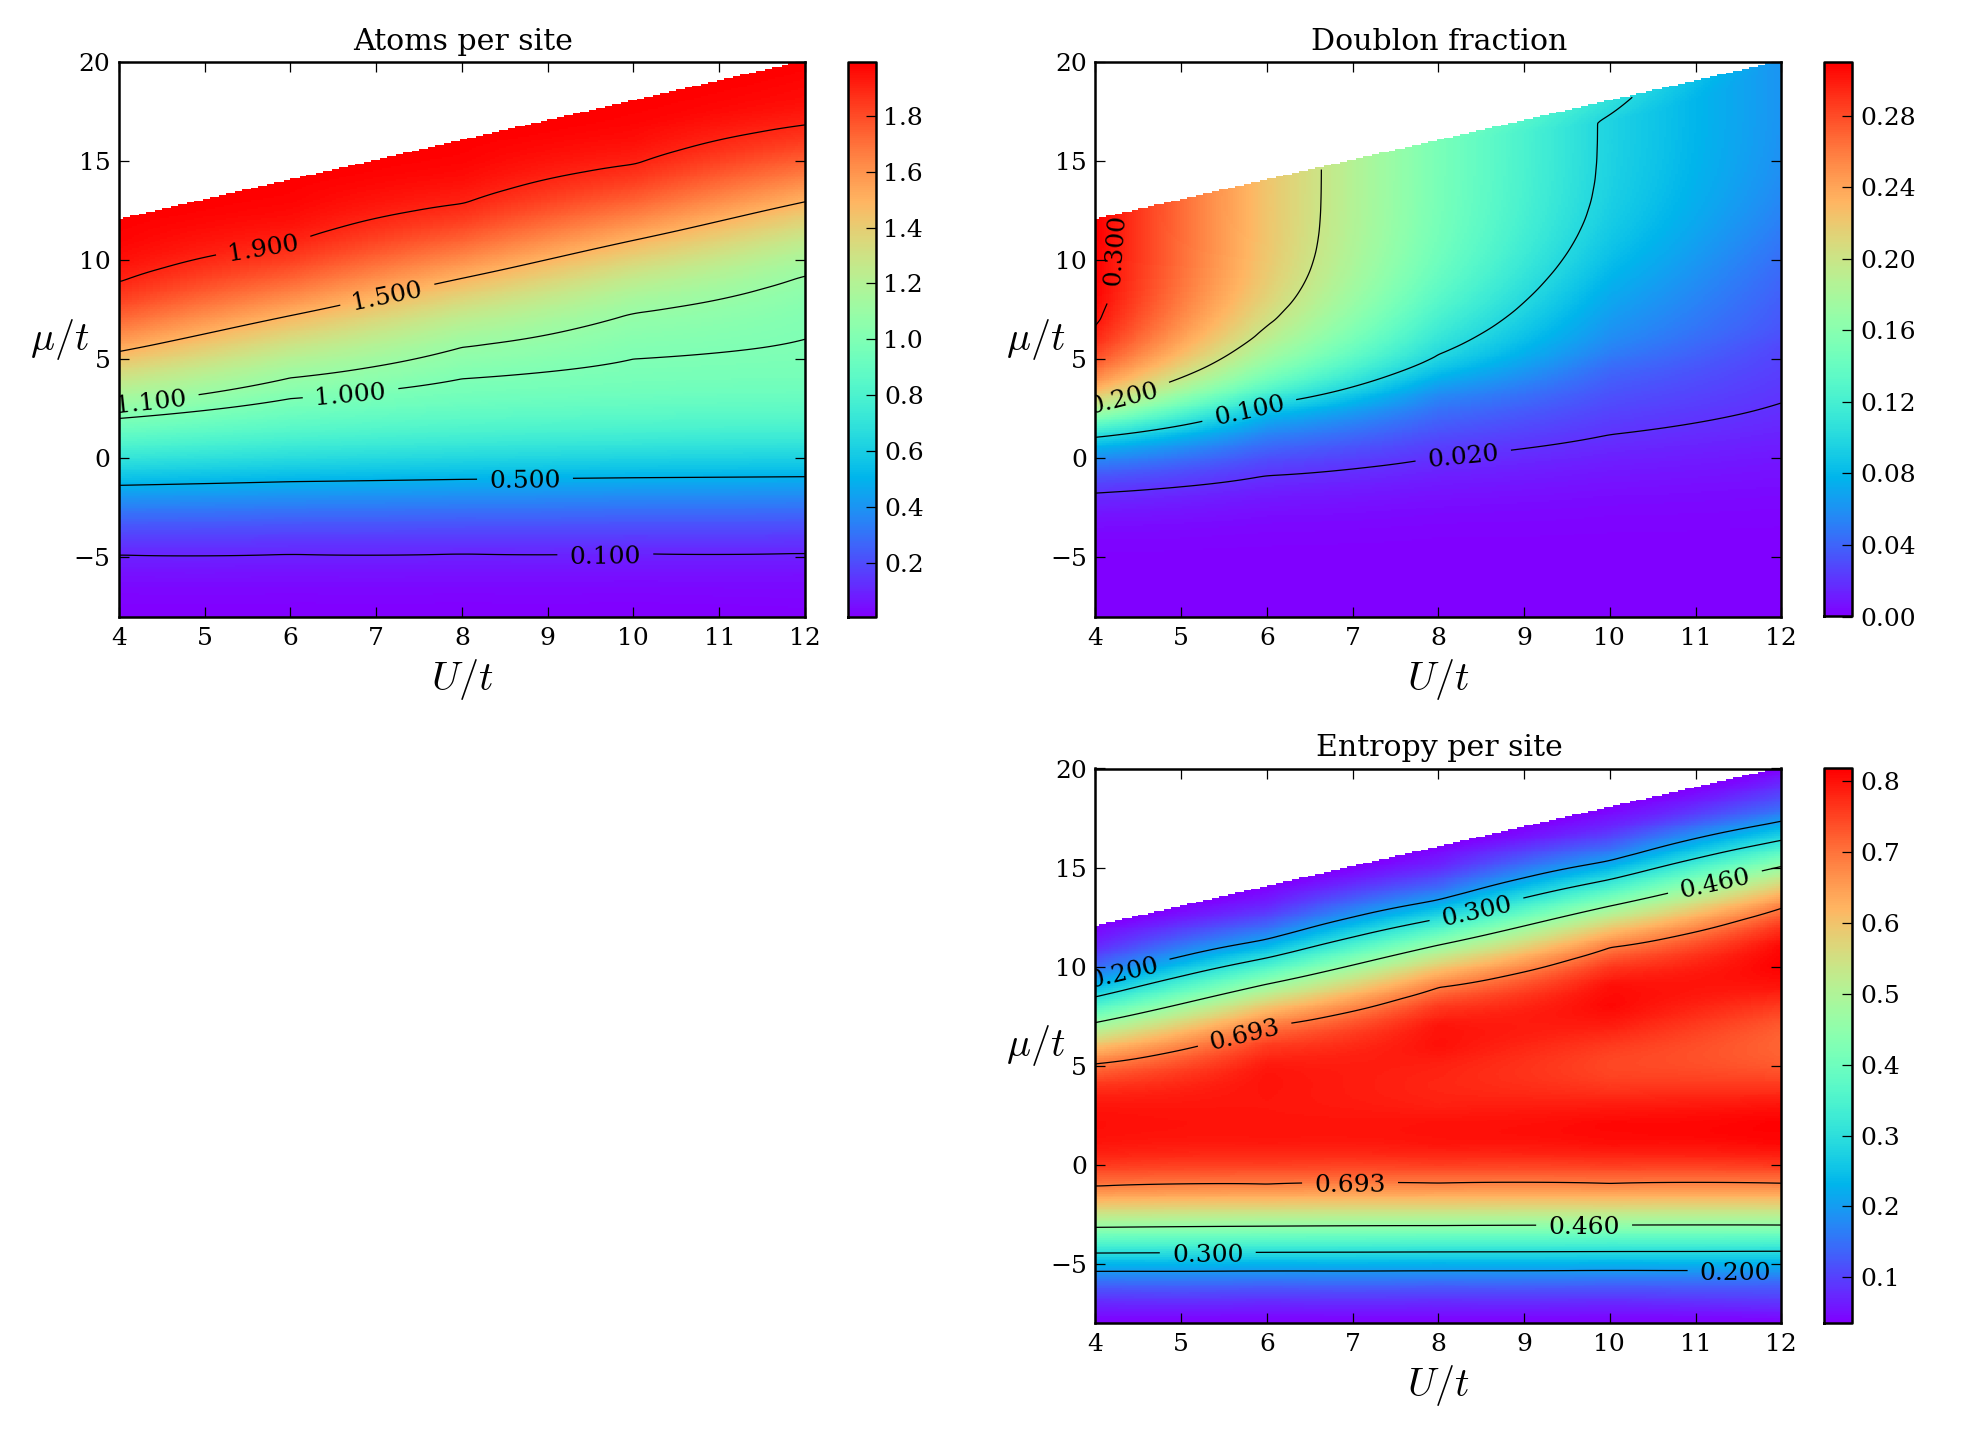
\includegraphics[width=\textwidth]{../HighT_figures/FUCHS_phasesT=10.png}
\caption[Low temperature phase diagram of the Fermi-Hubbard model]{\small
From~\cite{Fuchs2011}} \label{fig:fuchs10}
\end{figure}
   
\begin{figure}
\centering 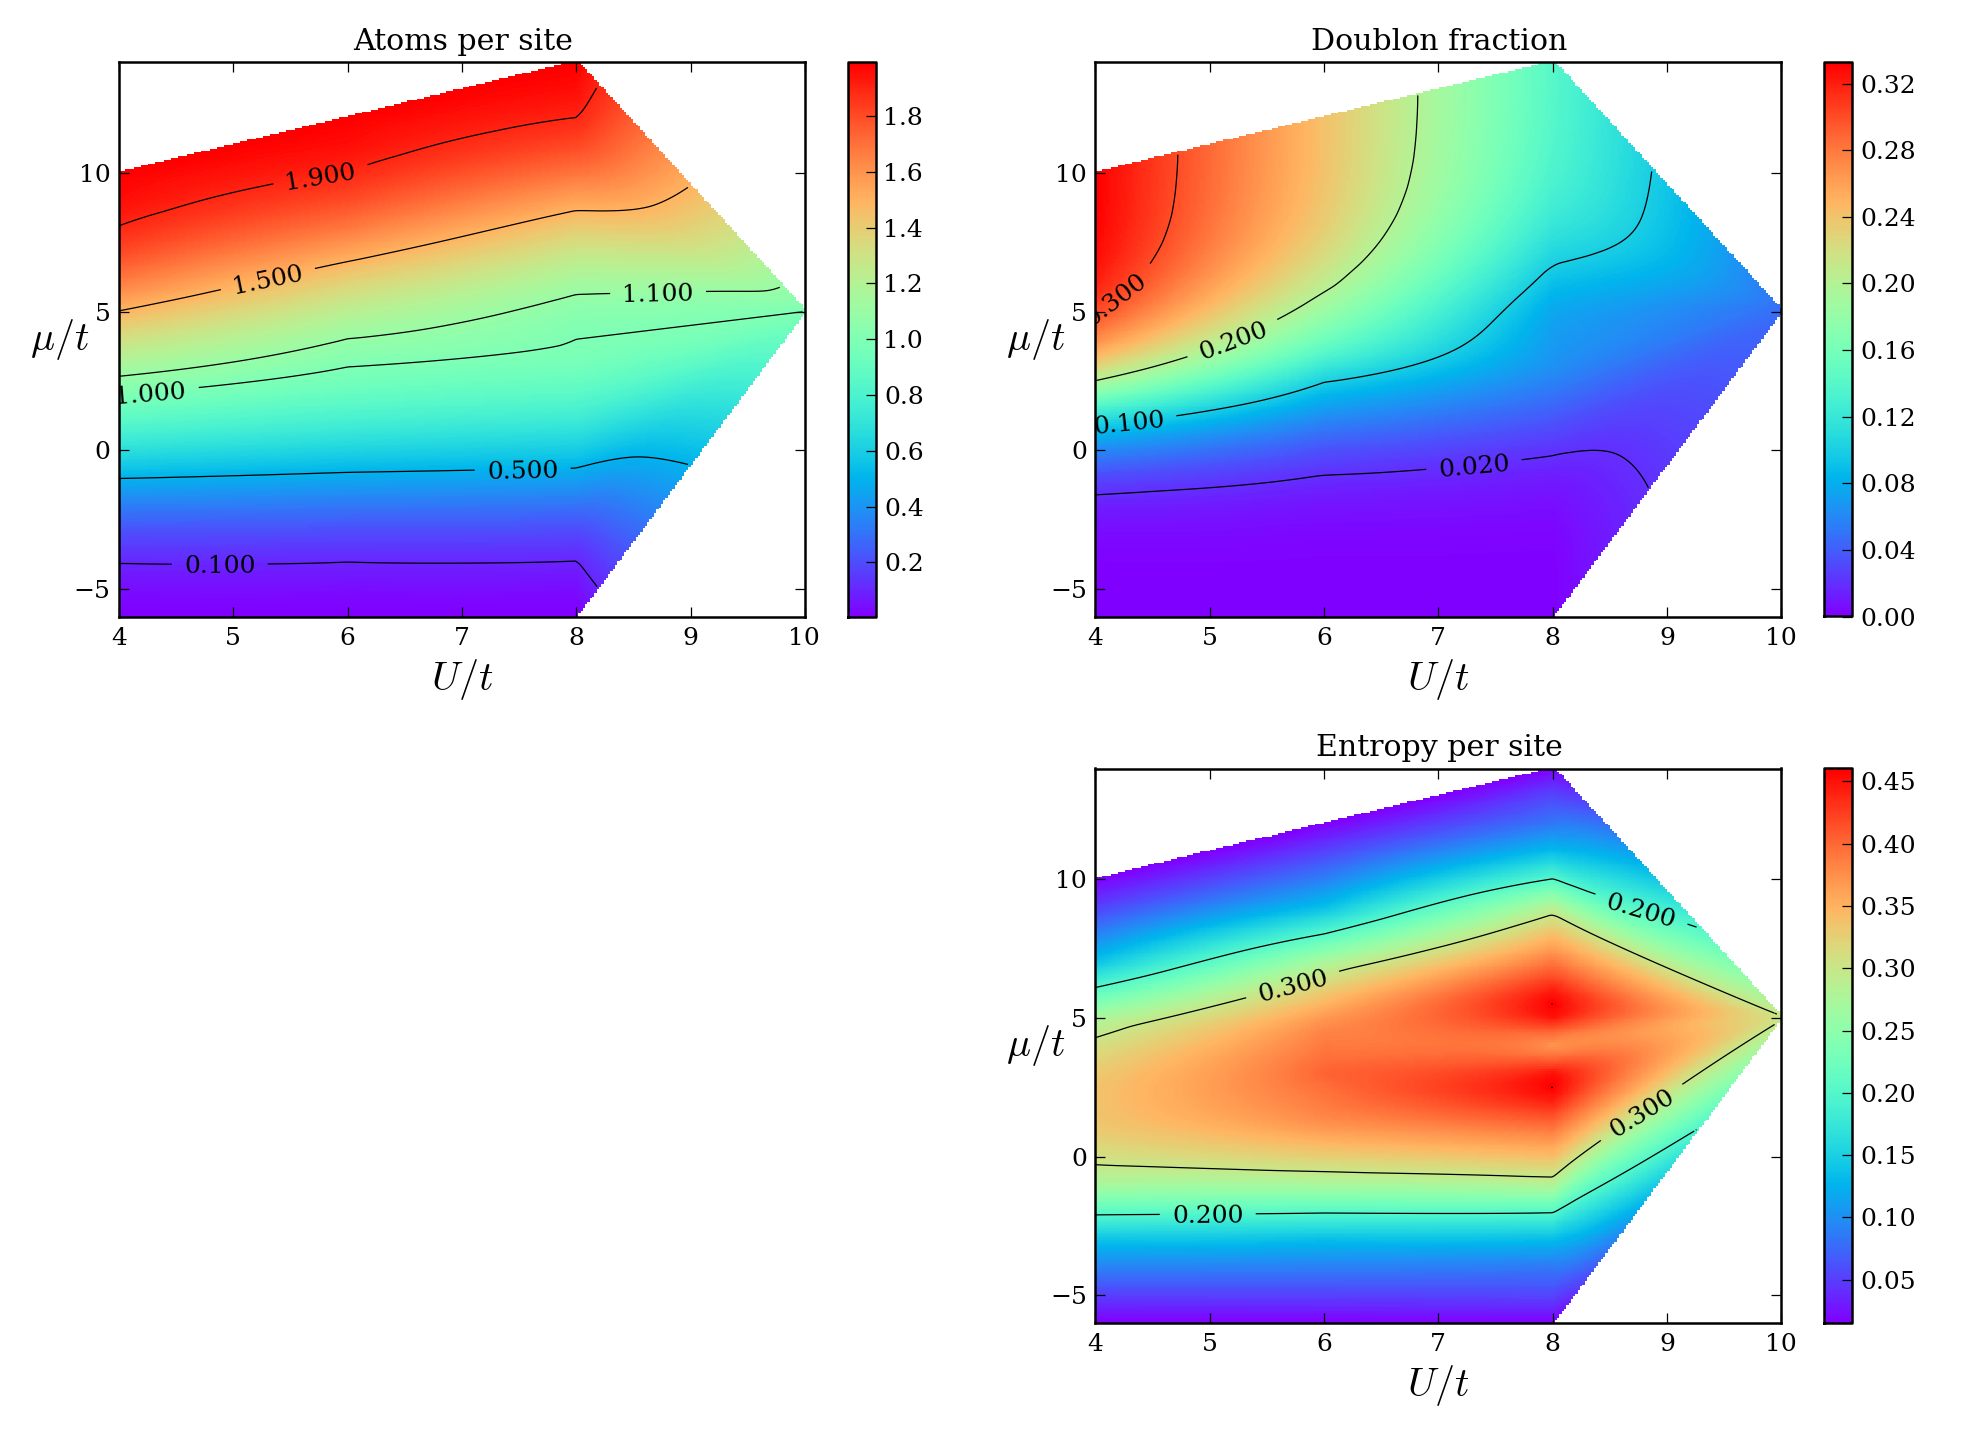
\includegraphics[width=\textwidth]{../HighT_figures/FUCHS_phasesT=3.png}
\caption[Low temperature phase diagram of the Fermi-Hubbard model]{\small
From~\cite{Fuchs2011}} \label{fig:fuchs10}
\end{figure}


\section{ Local density approximation }



The phase diagrams calculated in the two previous sections assume a homogeneous
lattice.  In our experiment the lattice has an underlying confining potential,
which can be dealt with by considering a local chemical potential at each point
in the trap given by
\begin{equation}
 \mu(\bv{r}) = \mu - V(\bv{r}) 
\end{equation}
An homogeneous lattice phase diagram can be used to obtain the local density,
local entropy, and local double occupancy at any point in our system by using
as inputs the local chemical potential,  the local value of the tunneling
matrix element and the local value of the on-site interaction.  

The methods used to calculate the phase diagrams are related to the validity of
the local density approximation.   We recall that in the high temperature
series expansion, the $n^{\text{th}}$  term corresponds to a particle staring
at a certain site, tunneling $n$ times and then coming back to its original
site.  If $\sqrt{n}$ becomes comparable to the lenght scale of variations in
the confining potential, then the local density would not be a suitable
description of the system, because in those $n$ steps the particle can sample a
very different confining potential.  

Similarly, in the cluster dynamical mean-field theory, results are obtained for
finite sized clusters of various sizes and then extrapolated to the infinite
size limit~\cite{Fuchs2011}.  At low temperatures, the system develops
long-range correlations, so large clusters are required to approximate the
system.   If the local site energy varies considerably over the size of a
cluster then the local density approximation will break down.   

\subsection{ Compensated lattice geometry }
 
 

\cite{PhysRevA.86.023606}

 

\bibliographystyle{osa}
\bibliography{lattice_lda}

\end{document}




